\documentclass{report}

%%%%%%%%%%%%%%%%%%%%%%%%%%%%%%%%%
% PACKAGE IMPORTS
%%%%%%%%%%%%%%%%%%%%%%%%%%%%%%%%%


\usepackage[tmargin=2cm,rmargin=1in,lmargin=1in,margin=0.85in,bmargin=2cm,footskip=.2in]{geometry}
\usepackage{amsmath,amsfonts,amsthm,amssymb,mathtools}
\usepackage[varbb]{newpxmath}
\usepackage{xfrac}
\usepackage[makeroom]{cancel}
\usepackage{mathtools}
\usepackage{bookmark}
\usepackage{enumitem}
\usepackage{hyperref,theoremref}
\hypersetup{
	pdftitle={Assignment},
	colorlinks=true, linkcolor=violet,
	bookmarksnumbered=true,
	bookmarksopen=true
}
\usepackage[most,many,breakable]{tcolorbox}
\usepackage{xcolor}
\usepackage{varwidth}
\usepackage{varwidth}
\usepackage{etoolbox}
%\usepackage{authblk}
\usepackage{nameref}
\usepackage{multicol,array}
\usepackage{tikz-cd}
\usepackage[ruled,vlined,linesnumbered]{algorithm2e}
\usepackage{comment} % enables the use of multi-line comments (\ifx \fi) 
\usepackage{import}
\usepackage{xifthen}
\usepackage{pdfpages}
\usepackage{transparent}
\usepackage{afterpage}

\newcommand\mycommfont[1]{\footnotesize\ttfamily\textcolor{violet}{#1}}
\SetCommentSty{mycommfont}
\newcommand{\incfig}[1]{%
    \def\svgwidth{\columnwidth}
    \import{./figures/}{#1.pdf_tex}
}

\usepackage{tikzsymbols}
\renewcommand\qedsymbol{$\Laughey$}


%\usepackage{import}
%\usepackage{xifthen}
%\usepackage{pdfpages}
%\usepackage{transparent}

%%%%%%%%%%%%%%%%%%%%%%%%%%%%%%
% TEX LIVE PACKAGES
%%%%%%%%%%%%%%%%%%%%%%%%%%%%%%

\usepackage[T1]{fontenc}
\usepackage{anyfontsize}

%%%%%%%%%%%%%%%%%%%%%%%%%%%%%%
% BLANK PAGE
%%%%%%%%%%%%%%%%%%%%%%%%%%%%%%

\newcommand\blankpage{%
    \null
    \thispagestyle{empty}%
    \addtocounter{page}{-1}%
    \newpage
}

%%%%%%%%%%%%%%%%%%%%%%%%%%%%%%
% SELF MADE COLORS
%%%%%%%%%%%%%%%%%%%%%%%%%%%%%%



\definecolor{myg}{RGB}{56, 140, 70}
\definecolor{myb}{RGB}{45, 111, 177}
\definecolor{myr}{RGB}{199, 68, 64}
\definecolor{mytheorembg}{HTML}{F2F2F9}
\definecolor{mytheoremfr}{HTML}{00007B}
\definecolor{mylenmabg}{HTML}{FFFAF8}
\definecolor{mylenmafr}{HTML}{983b0f}
\definecolor{mypropbg}{HTML}{f2fbfc}
\definecolor{mypropfr}{HTML}{191971}
\definecolor{myexamplebg}{HTML}{F2FBF8}
\definecolor{myexamplefr}{HTML}{88D6D1}
\definecolor{myexampleti}{HTML}{2A7F7F}
\definecolor{mydefinitbg}{HTML}{E5E5FF}
\definecolor{mydefinitfr}{HTML}{3F3FA3}
\definecolor{notesred}{RGB}{0,162,0}
\definecolor{myp}{RGB}{197, 92, 212}
\definecolor{mygr}{HTML}{2C3338}
\definecolor{myred}{RGB}{127,0,0}
\definecolor{myyellow}{RGB}{169,121,69}
\definecolor{myexercisebg}{HTML}{F2FBF8}
\definecolor{myexercisefg}{HTML}{88D6D1}


%%%%%%%%%%%%%%%%%%%%%%%%%%%%
% TCOLORBOX SETUPS
%%%%%%%%%%%%%%%%%%%%%%%%%%%%

\setlength{\parindent}{1cm}
%================================
% THEOREM BOX
%================================

\tcbuselibrary{theorems,skins,hooks}
\newtcbtheorem[number within=section]{Theorem}{Teorema}
{%
	enhanced,
	breakable,
	colback = mytheorembg,
	frame hidden,
	boxrule = 0sp,
	borderline west = {2pt}{0pt}{mytheoremfr},
	sharp corners,
	detach title,
	before upper = \tcbtitle\par\smallskip,
	coltitle = mytheoremfr,
	fonttitle = \bfseries\sffamily,
	description font = \mdseries,
	separator sign none,
	segmentation style={solid, mytheoremfr},
}
{th}

\tcbuselibrary{theorems,skins,hooks}
\newtcbtheorem[number within=chapter]{theorem}{Theorem}
{%
	enhanced,
	breakable,
	colback = mytheorembg,
	frame hidden,
	boxrule = 0sp,
	borderline west = {2pt}{0pt}{mytheoremfr},
	sharp corners,
	detach title,
	before upper = \tcbtitle\par\smallskip,
	coltitle = mytheoremfr,
	fonttitle = \bfseries\sffamily,
	description font = \mdseries,
	separator sign none,
	segmentation style={solid, mytheoremfr},
}
{th}


\tcbuselibrary{theorems,skins,hooks}
\newtcolorbox{Theoremcon}
{%
	enhanced
	,breakable
	,colback = mytheorembg
	,frame hidden
	,boxrule = 0sp
	,borderline west = {2pt}{0pt}{mytheoremfr}
	,sharp corners
	,description font = \mdseries
	,separator sign none
}

%================================
% Corollery
%================================
\tcbuselibrary{theorems,skins,hooks}
\newtcbtheorem[number within=section]{Corollary}{Corollario}
{%
	enhanced
	,breakable
	,colback = myp!10
	,frame hidden
	,boxrule = 0sp
	,borderline west = {2pt}{0pt}{myp!85!black}
	,sharp corners
	,detach title
	,before upper = \tcbtitle\par\smallskip
	,coltitle = myp!85!black
	,fonttitle = \bfseries\sffamily
	,description font = \mdseries
	,separator sign none
	,segmentation style={solid, myp!85!black}
}
{th}
\tcbuselibrary{theorems,skins,hooks}
\newtcbtheorem[number within=chapter]{corollary}{Corollary}
{%
	enhanced
	,breakable
	,colback = myp!10
	,frame hidden
	,boxrule = 0sp
	,borderline west = {2pt}{0pt}{myp!85!black}
	,sharp corners
	,detach title
	,before upper = \tcbtitle\par\smallskip
	,coltitle = myp!85!black
	,fonttitle = \bfseries\sffamily
	,description font = \mdseries
	,separator sign none
	,segmentation style={solid, myp!85!black}
}
{th}


%================================
% LENMA
%================================

\tcbuselibrary{theorems,skins,hooks}
\newtcbtheorem[number within=section]{Lenma}{Lenma}
{%
	enhanced,
	breakable,
	colback = mylenmabg,
	frame hidden,
	boxrule = 0sp,
	borderline west = {2pt}{0pt}{mylenmafr},
	sharp corners,
	detach title,
	before upper = \tcbtitle\par\smallskip,
	coltitle = mylenmafr,
	fonttitle = \bfseries\sffamily,
	description font = \mdseries,
	separator sign none,
	segmentation style={solid, mylenmafr},
}
{th}

\tcbuselibrary{theorems,skins,hooks}
\newtcbtheorem[number within=chapter]{lenma}{Lenma}
{%
	enhanced,
	breakable,
	colback = mylenmabg,
	frame hidden,
	boxrule = 0sp,
	borderline west = {2pt}{0pt}{mylenmafr},
	sharp corners,
	detach title,
	before upper = \tcbtitle\par\smallskip,
	coltitle = mylenmafr,
	fonttitle = \bfseries\sffamily,
	description font = \mdseries,
	separator sign none,
	segmentation style={solid, mylenmafr},
}
{th}


%================================
% PROPOSITION
%================================

\tcbuselibrary{theorems,skins,hooks}
\newtcbtheorem[number within=section]{Prop}{Proposition}
{%
	enhanced,
	breakable,
	colback = mypropbg,
	frame hidden,
	boxrule = 0sp,
	borderline west = {2pt}{0pt}{mypropfr},
	sharp corners,
	detach title,
	before upper = \tcbtitle\par\smallskip,
	coltitle = mypropfr,
	fonttitle = \bfseries\sffamily,
	description font = \mdseries,
	separator sign none,
	segmentation style={solid, mypropfr},
}
{th}

\tcbuselibrary{theorems,skins,hooks}
\newtcbtheorem[number within=chapter]{prop}{Proposition}
{%
	enhanced,
	breakable,
	colback = mypropbg,
	frame hidden,
	boxrule = 0sp,
	borderline west = {2pt}{0pt}{mypropfr},
	sharp corners,
	detach title,
	before upper = \tcbtitle\par\smallskip,
	coltitle = mypropfr,
	fonttitle = \bfseries\sffamily,
	description font = \mdseries,
	separator sign none,
	segmentation style={solid, mypropfr},
}
{th}


%================================
% CLAIM
%================================

\tcbuselibrary{theorems,skins,hooks}
\newtcbtheorem[number within=section]{claim}{Claim}
{%
	enhanced
	,breakable
	,colback = myg!10
	,frame hidden
	,boxrule = 0sp
	,borderline west = {2pt}{0pt}{myg}
	,sharp corners
	,detach title
	,before upper = \tcbtitle\par\smallskip
	,coltitle = myg!85!black
	,fonttitle = \bfseries\sffamily
	,description font = \mdseries
	,separator sign none
	,segmentation style={solid, myg!85!black}
}
{th}



%================================
% Exercise
%================================

\tcbuselibrary{theorems,skins,hooks}
\newtcbtheorem[number within=section]{Exercise}{Exercise}
{%
	enhanced,
	breakable,
	colback = myexercisebg,
	frame hidden,
	boxrule = 0sp,
	borderline west = {2pt}{0pt}{myexercisefg},
	sharp corners,
	detach title,
	before upper = \tcbtitle\par\smallskip,
	coltitle = myexercisefg,
	fonttitle = \bfseries\sffamily,
	description font = \mdseries,
	separator sign none,
	segmentation style={solid, myexercisefg},
}
{th}

\tcbuselibrary{theorems,skins,hooks}
\newtcbtheorem[number within=chapter]{exercise}{Exercise}
{%
	enhanced,
	breakable,
	colback = myexercisebg,
	frame hidden,
	boxrule = 0sp,
	borderline west = {2pt}{0pt}{myexercisefg},
	sharp corners,
	detach title,
	before upper = \tcbtitle\par\smallskip,
	coltitle = myexercisefg,
	fonttitle = \bfseries\sffamily,
	description font = \mdseries,
	separator sign none,
	segmentation style={solid, myexercisefg},
}
{th}

%================================
% EXAMPLE BOX
%================================

\newtcbtheorem[number within=section]{Example}{Esempio}
{%
	colback = myexamplebg
	,breakable
	,colframe = myexamplefr
	,coltitle = myexampleti
	,boxrule = 1pt
	,sharp corners
	,detach title
	,before upper=\tcbtitle\par\smallskip
	,fonttitle = \bfseries
	,description font = \mdseries
	,separator sign none
	,description delimiters parenthesis
}
{ex}

\newtcbtheorem[number within=chapter]{example}{Esempio}
{%
	colback = myexamplebg
	,breakable
	,colframe = myexamplefr
	,coltitle = myexampleti
	,boxrule = 1pt
	,sharp corners
	,detach title
	,before upper=\tcbtitle\par\smallskip
	,fonttitle = \bfseries
	,description font = \mdseries
	,separator sign none
	,description delimiters parenthesis
}
{ex}

%================================
% DEFINITION BOX
%================================

\newtcbtheorem[number within=section]{Definizione}{Definizione}{enhanced,
	before skip=2mm,after skip=2mm, colback=red!5,colframe=red!80!black,boxrule=0.5mm,
	attach boxed title to top left={xshift=1cm,yshift*=1mm-\tcboxedtitleheight}, varwidth boxed title*=-3cm,
	boxed title style={frame code={
					\path[fill=tcbcolback]
					([yshift=-1mm,xshift=-1mm]frame.north west)
					arc[start angle=0,end angle=180,radius=1mm]
					([yshift=-1mm,xshift=1mm]frame.north east)
					arc[start angle=180,end angle=0,radius=1mm];
					\path[left color=tcbcolback!60!black,right color=tcbcolback!60!black,
						middle color=tcbcolback!80!black]
					([xshift=-2mm]frame.north west) -- ([xshift=2mm]frame.north east)
					[rounded corners=1mm]-- ([xshift=1mm,yshift=-1mm]frame.north east)
					-- (frame.south east) -- (frame.south west)
					-- ([xshift=-1mm,yshift=-1mm]frame.north west)
					[sharp corners]-- cycle;
				},interior engine=empty,
		},
	fonttitle=\bfseries,
	title={#2},#1}{def}
\newtcbtheorem[number within=chapter]{definizione}{Definizione}{enhanced,
	before skip=2mm,after skip=2mm, colback=red!5,colframe=red!80!black,boxrule=0.5mm,
	attach boxed title to top left={xshift=1cm,yshift*=1mm-\tcboxedtitleheight}, varwidth boxed title*=-3cm,
	boxed title style={frame code={
					\path[fill=tcbcolback]
					([yshift=-1mm,xshift=-1mm]frame.north west)
					arc[start angle=0,end angle=180,radius=1mm]
					([yshift=-1mm,xshift=1mm]frame.north east)
					arc[start angle=180,end angle=0,radius=1mm];
					\path[left color=tcbcolback!60!black,right color=tcbcolback!60!black,
						middle color=tcbcolback!80!black]
					([xshift=-2mm]frame.north west) -- ([xshift=2mm]frame.north east)
					[rounded corners=1mm]-- ([xshift=1mm,yshift=-1mm]frame.north east)
					-- (frame.south east) -- (frame.south west)
					-- ([xshift=-1mm,yshift=-1mm]frame.north west)
					[sharp corners]-- cycle;
				},interior engine=empty,
		},
	fonttitle=\bfseries,
	title={#2},#1}{def}



%================================
% Solution BOX
%================================

\makeatletter
\newtcbtheorem{question}{Question}{enhanced,
	breakable,
	colback=white,
	colframe=myb!80!black,
	attach boxed title to top left={yshift*=-\tcboxedtitleheight},
	fonttitle=\bfseries,
	title={#2},
	boxed title size=title,
	boxed title style={%
			sharp corners,
			rounded corners=northwest,
			colback=tcbcolframe,
			boxrule=0pt,
		},
	underlay boxed title={%
			\path[fill=tcbcolframe] (title.south west)--(title.south east)
			to[out=0, in=180] ([xshift=5mm]title.east)--
			(title.center-|frame.east)
			[rounded corners=\kvtcb@arc] |-
			(frame.north) -| cycle;
		},
	#1
}{def}
\makeatother

%================================
% SOLUTION BOX
%================================

\makeatletter
\newtcolorbox{solution}{enhanced,
	breakable,
	colback=white,
	colframe=myg!80!black,
	attach boxed title to top left={yshift*=-\tcboxedtitleheight},
	title=Solution,
	boxed title size=title,
	boxed title style={%
			sharp corners,
			rounded corners=northwest,
			colback=tcbcolframe,
			boxrule=0pt,
		},
	underlay boxed title={%
			\path[fill=tcbcolframe] (title.south west)--(title.south east)
			to[out=0, in=180] ([xshift=5mm]title.east)--
			(title.center-|frame.east)
			[rounded corners=\kvtcb@arc] |-
			(frame.north) -| cycle;
		},
}
\makeatother

%================================
% Question BOX
%================================

\makeatletter
\newtcbtheorem{qstion}{Question}{enhanced,
	breakable,
	colback=white,
	colframe=mygr,
	attach boxed title to top left={yshift*=-\tcboxedtitleheight},
	fonttitle=\bfseries,
	title={#2},
	boxed title size=title,
	boxed title style={%
			sharp corners,
			rounded corners=northwest,
			colback=tcbcolframe,
			boxrule=0pt,
		},
	underlay boxed title={%
			\path[fill=tcbcolframe] (title.south west)--(title.south east)
			to[out=0, in=180] ([xshift=5mm]title.east)--
			(title.center-|frame.east)
			[rounded corners=\kvtcb@arc] |-
			(frame.north) -| cycle;
		},
	#1
}{def}
\makeatother

\newtcbtheorem[number within=chapter]{wconc}{Wrong Concept}{
	breakable,
	enhanced,
	colback=white,
	colframe=myr,
	arc=0pt,
	outer arc=0pt,
	fonttitle=\bfseries\sffamily\large,
	colbacktitle=myr,
	attach boxed title to top left={},
	boxed title style={
			enhanced,
			skin=enhancedfirst jigsaw,
			arc=3pt,
			bottom=0pt,
			interior style={fill=myr}
		},
	#1
}{def}



%================================
% NOTE BOX
%================================

\usetikzlibrary{arrows,calc,shadows.blur}
\tcbuselibrary{skins}
\newtcolorbox{note}[1][]{%
	enhanced jigsaw,
	colback=gray!20!white,%
	colframe=gray!80!black,
	size=small,
	boxrule=1pt,
	title=\textbf{Note:-},
	halign title=flush center,
	coltitle=black,
	breakable,
	drop shadow=black!50!white,
	attach boxed title to top left={xshift=1cm,yshift=-\tcboxedtitleheight/2,yshifttext=-\tcboxedtitleheight/2},
	minipage boxed title=1.5cm,
	boxed title style={%
			colback=white,
			size=fbox,
			boxrule=1pt,
			boxsep=2pt,
			underlay={%
					\coordinate (dotA) at ($(interior.west) + (-0.5pt,0)$);
					\coordinate (dotB) at ($(interior.east) + (0.5pt,0)$);
					\begin{scope}
						\clip (interior.north west) rectangle ([xshift=3ex]interior.east);
						\filldraw [white, blur shadow={shadow opacity=60, shadow yshift=-.75ex}, rounded corners=2pt] (interior.north west) rectangle (interior.south east);
					\end{scope}
					\begin{scope}[gray!80!black]
						\fill (dotA) circle (2pt);
						\fill (dotB) circle (2pt);
					\end{scope}
				},
		},
	#1,
}

%%%%%%%%%%%%%%%%%%%%%%%%%%%%%%
% SELF MADE COMMANDS
%%%%%%%%%%%%%%%%%%%%%%%%%%%%%%


\newcommand{\thm}[2]{\begin{Theorem}{#1}{}#2\end{Theorem}}
\newcommand{\cor}[2]{\begin{Corollary}{#1}{}#2\end{Corollary}}
\newcommand{\mlenma}[2]{\begin{Lenma}{#1}{}#2\end{Lenma}}
\newcommand{\mprop}[2]{\begin{Prop}{#1}{}#2\end{Prop}}
\newcommand{\clm}[3]{\begin{claim}{#1}{#2}#3\end{claim}}
\newcommand{\wc}[2]{\begin{wconc}{#1}{}\setlength{\parindent}{1cm}#2\end{wconc}}
\newcommand{\thmcon}[1]{\begin{Theoremcon}{#1}\end{Theoremcon}}
\newcommand{\ex}[2]{\begin{Example}{#1}{}#2\end{Example}}
\newcommand{\dfn}[2]{\begin{Definizione}[colbacktitle=red!75!black]{#1}{}#2\end{Definizione}}
\newcommand{\dfnc}[2]{\begin{definizione}[colbacktitle=red!75!black]{#1}{}#2\end{definizione}}
\newcommand{\qs}[2]{\begin{question}{#1}{}#2\end{question}}
\newcommand{\pf}[2]{\begin{myproof}[#1]#2\end{myproof}}
\newcommand{\nt}[1]{\begin{note}#1\end{note}}

\newcommand*\circled[1]{\tikz[baseline=(char.base)]{
		\node[shape=circle,draw,inner sep=1pt] (char) {#1};}}
\newcommand\getcurrentref[1]{%
	\ifnumequal{\value{#1}}{0}
	{??}
	{\the\value{#1}}%
}
\newcommand{\getCurrentSectionNumber}{\getcurrentref{section}}
\newenvironment{myproof}[1][\proofname]{%
	\proof[\bfseries #1: ]%
}{\endproof}

\newcommand{\mclm}[2]{\begin{myclaim}[#1]#2\end{myclaim}}
\newenvironment{myclaim}[1][\claimname]{\proof[\bfseries #1: ]}{}

\newcounter{mylabelcounter}

\makeatletter
\newcommand{\setword}[2]{%
	\phantomsection
	#1\def\@currentlabel{\unexpanded{#1}}\label{#2}%
}
\makeatother




\tikzset{
	symbol/.style={
			draw=none,
			every to/.append style={
					edge node={node [sloped, allow upside down, auto=false]{$#1$}}}
		}
}


% deliminators
\DeclarePairedDelimiter{\abs}{\lvert}{\rvert}
\DeclarePairedDelimiter{\norm}{\lVert}{\rVert}

\DeclarePairedDelimiter{\ceil}{\lceil}{\rceil}
\DeclarePairedDelimiter{\floor}{\lfloor}{\rfloor}
\DeclarePairedDelimiter{\round}{\lfloor}{\rceil}

\newsavebox\diffdbox
\newcommand{\slantedromand}{{\mathpalette\makesl{d}}}
\newcommand{\makesl}[2]{%
\begingroup
\sbox{\diffdbox}{$\mathsurround=0pt#1\mathrm{#2}$}%
\pdfsave
\pdfsetmatrix{1 0 0.2 1}%
\rlap{\usebox{\diffdbox}}%
\pdfrestore
\hskip\wd\diffdbox
\endgroup
}
\newcommand{\dd}[1][]{\ensuremath{\mathop{}\!\ifstrempty{#1}{%
\slantedromand\@ifnextchar^{\hspace{0.2ex}}{\hspace{0.1ex}}}%
{\slantedromand\hspace{0.2ex}^{#1}}}}
\ProvideDocumentCommand\dv{o m g}{%
  \ensuremath{%
    \IfValueTF{#3}{%
      \IfNoValueTF{#1}{%
        \frac{\dd #2}{\dd #3}%
      }{%
        \frac{\dd^{#1} #2}{\dd #3^{#1}}%
      }%
    }{%
      \IfNoValueTF{#1}{%
        \frac{\dd}{\dd #2}%
      }{%
        \frac{\dd^{#1}}{\dd #2^{#1}}%
      }%
    }%
  }%
}
\providecommand*{\pdv}[3][]{\frac{\partial^{#1}#2}{\partial#3^{#1}}}
%  - others
\DeclareMathOperator{\Lap}{\mathcal{L}}
\DeclareMathOperator{\Var}{Var} % varience
\DeclareMathOperator{\Cov}{Cov} % covarience
\DeclareMathOperator{\E}{E} % expected

% Since the amsthm package isn't loaded

% I prefer the slanted \leq
\let\oldleq\leq % save them in case they're every wanted
\let\oldgeq\geq
\renewcommand{\leq}{\leqslant}
\renewcommand{\geq}{\geqslant}

% % redefine matrix env to allow for alignment, use r as default
% \renewcommand*\env@matrix[1][r]{\hskip -\arraycolsep
%     \let\@ifnextchar\new@ifnextchar
%     \array{*\c@MaxMatrixCols #1}}


%\usepackage{framed}
%\usepackage{titletoc}
%\usepackage{etoolbox}
%\usepackage{lmodern}


%\patchcmd{\tableofcontents}{\contentsname}{\sffamily\contentsname}{}{}

%\renewenvironment{leftbar}
%{\def\FrameCommand{\hspace{6em}%
%		{\color{myyellow}\vrule width 2pt depth 6pt}\hspace{1em}}%
%	\MakeFramed{\parshape 1 0cm \dimexpr\textwidth-6em\relax\FrameRestore}\vskip2pt%
%}
%{\endMakeFramed}

%\titlecontents{chapter}
%[0em]{\vspace*{2\baselineskip}}
%{\parbox{4.5em}{%
%		\hfill\Huge\sffamily\bfseries\color{myred}\thecontentspage}%
%	\vspace*{-2.3\baselineskip}\leftbar\textsc{\small\chaptername~\thecontentslabel}\\\sffamily}
%{}{\endleftbar}
%\titlecontents{section}
%[8.4em]
%{\sffamily\contentslabel{3em}}{}{}
%{\hspace{0.5em}\nobreak\itshape\color{myred}\contentspage}
%\titlecontents{subsection}
%[8.4em]
%{\sffamily\contentslabel{3em}}{}{}  
%{\hspace{0.5em}\nobreak\itshape\color{myred}\contentspage}



%%%%%%%%%%%%%%%%%%%%%%%%%%%%%%%%%%%%%%%%%%%
% TABLE OF CONTENTS
%%%%%%%%%%%%%%%%%%%%%%%%%%%%%%%%%%%%%%%%%%%

\usepackage{tikz}
\definecolor{doc}{RGB}{0,60,110}
\usepackage{titletoc}
\contentsmargin{0cm}
\titlecontents{chapter}[3.7pc]
{\addvspace{30pt}%
	\begin{tikzpicture}[remember picture, overlay]%
		\draw[fill=violet,draw=violet] (-7.3,-.1) rectangle (-0.5,.5);%
		\pgftext[left,x=-3.7cm,y=0.2cm]{\color{white}\Large\sc\bfseries Capitolo\ \thecontentslabel};%
	\end{tikzpicture}\color{violet}\large\sc\bfseries}%
{}
{}
{\;\titlerule\;\large\sc\bfseries Pagina \thecontentspage
	\begin{tikzpicture}[remember picture, overlay]
		\draw[fill=violet,draw=violet] (2pt,0) rectangle (4,0.1pt);
	\end{tikzpicture}}%
\titlecontents{section}[3.7pc]
{\addvspace{2pt}}
{\contentslabel[\thecontentslabel]{2pc}}
{}
{\hfill\small \thecontentspage}
[]
\titlecontents*{subsection}[3.7pc]
{\addvspace{-1pt}\small}
{}
{}
{\ --- \small\thecontentspage}
[ \textbullet\ ][]

\makeatletter
\renewcommand{\chaptername}{Capitolo}
\renewcommand{\tableofcontents}{%
	\chapter*{%
	  \vspace*{-20\p@}%
	  \begin{tikzpicture}[remember picture, overlay]%
		  \pgftext[right,x=15cm,y=0.2cm]{\color{violet}\Huge\sc\bfseries \contentsname};%
		  \draw[fill=violet,draw=violet] (13,-.75) rectangle (20,1);%
		  \clip (13,-.75) rectangle (20,1);
		  \pgftext[right,x=15cm,y=0.2cm]{\color{white}\Huge\sc\bfseries \contentsname};%
	  \end{tikzpicture}}%
	\@starttoc{toc}}
\makeatother

%%%%%%%%%%%%%%%%%%%%%%%%%%%%%%%%%%%%%%%%%%%
% HYPERLINK
%%%%%%%%%%%%%%%%%%%%%%%%%%%%%%%%%%%%%%%%%%%

\hypersetup{
    colorlinks,
    citecolor=black,
    filecolor=black,
    linkcolor=black,
    urlcolor=black
}
%From M275 "Topology" at SJSU
\newcommand{\id}{\mathrm{id}}
\newcommand{\taking}[1]{\xrightarrow{#1}}
\newcommand{\inv}{^{-1}}

%From M170 "Introduction to Graph Theory" at SJSU
\DeclareMathOperator{\diam}{diam}
\DeclareMathOperator{\ord}{ord}
\newcommand{\defeq}{\overset{\mathrm{def}}{=}}

%From the USAMO .tex files
\newcommand{\ts}{\textsuperscript}
\newcommand{\dg}{^\circ}
\newcommand{\ii}{\item}

% % From Math 55 and Math 145 at Harvard
% \newenvironment{subproof}[1][Proof]{%
% \begin{proof}[#1] \renewcommand{\qedsymbol}{$\blacksquare$}}%
% {\end{proof}}

\newcommand{\ac}{\Leftrightarrow_\alpha}
\newcommand{\br}{\rightarrow_\beta}
\newcommand{\er}{\rightarrow_\eta}
\newcommand{\liff}{\leftrightarrow}
\newcommand{\lthen}{\rightarrow}
\newcommand{\opname}{\operatorname}
\newcommand{\surjto}{\twoheadrightarrow}
\newcommand{\injto}{\hookrightarrow}
\newcommand{\On}{\mathrm{On}} % ordinals
\DeclareMathOperator{\img}{im} % Image
\DeclareMathOperator{\Img}{Im} % Image
\DeclareMathOperator{\coker}{coker} % Cokernel
\DeclareMathOperator{\Coker}{Coker} % Cokernel
\DeclareMathOperator{\Ker}{Ker} % Kernel
\DeclareMathOperator{\rank}{rank}
\DeclareMathOperator{\Spec}{Spec} % spectrum
\DeclareMathOperator{\Tr}{Tr} % trace
\DeclareMathOperator{\pr}{pr} % projection
\DeclareMathOperator{\ext}{ext} % extension
\DeclareMathOperator{\pred}{pred} % predecessor
\DeclareMathOperator{\dom}{dom} % domain
\DeclareMathOperator{\ran}{ran} % range
\DeclareMathOperator{\Hom}{Hom} % homomorphism
\DeclareMathOperator{\Mor}{Mor} % morphisms
\DeclareMathOperator{\End}{End} % endomorphism

\newcommand{\eps}{\epsilon}
\newcommand{\veps}{\varepsilon}
\newcommand{\ol}{\overline}
\newcommand{\ul}{\underline}
\newcommand{\wt}{\widetilde}
\newcommand{\wh}{\widehat}
\newcommand{\vocab}[1]{\textbf{\color{blue} #1}}
\providecommand{\half}{\frac{1}{2}}
\newcommand{\dang}{\measuredangle} %% Directed angle
\newcommand{\ray}[1]{\overrightarrow{#1}}
\newcommand{\seg}[1]{\overline{#1}}
\newcommand{\arc}[1]{\wideparen{#1}}
\DeclareMathOperator{\cis}{cis}
\DeclareMathOperator*{\lcm}{lcm}
\DeclareMathOperator*{\argmin}{arg min}
\DeclareMathOperator*{\argmax}{arg max}
\newcommand{\cycsum}{\sum_{\mathrm{cyc}}}
\newcommand{\symsum}{\sum_{\mathrm{sym}}}
\newcommand{\cycprod}{\prod_{\mathrm{cyc}}}
\newcommand{\symprod}{\prod_{\mathrm{sym}}}
\newcommand{\Qed}{\begin{flushright}\qed\end{flushright}}
\newcommand{\parinn}{\setlength{\parindent}{1cm}}
\newcommand{\parinf}{\setlength{\parindent}{0cm}}
% \newcommand{\norm}{\|\cdot\|}
\newcommand{\inorm}{\norm_{\infty}}
\newcommand{\opensets}{\{V_{\alpha}\}_{\alpha\in I}}
\newcommand{\oset}{V_{\alpha}}
\newcommand{\opset}[1]{V_{\alpha_{#1}}}
\newcommand{\lub}{\text{lub}}
\newcommand{\del}[2]{\frac{\partial #1}{\partial #2}}
\newcommand{\Del}[3]{\frac{\partial^{#1} #2}{\partial^{#1} #3}}
\newcommand{\deld}[2]{\dfrac{\partial #1}{\partial #2}}
\newcommand{\Deld}[3]{\dfrac{\partial^{#1} #2}{\partial^{#1} #3}}
\newcommand{\lm}{\lambda}
\newcommand{\uin}{\mathbin{\rotatebox[origin=c]{90}{$\in$}}}
\newcommand{\usubset}{\mathbin{\rotatebox[origin=c]{90}{$\subset$}}}
\newcommand{\lt}{\left}
\newcommand{\rt}{\right}
\newcommand{\bs}[1]{\boldsymbol{#1}}
\newcommand{\exs}{\exists}
\newcommand{\st}{\strut}
\newcommand{\dps}[1]{\displaystyle{#1}}

\newcommand{\sol}{\setlength{\parindent}{0cm}\textbf{\textit{Solution:}}\setlength{\parindent}{1cm} }
\newcommand{\solve}[1]{\setlength{\parindent}{0cm}\textbf{\textit{Solution: }}\setlength{\parindent}{1cm}#1 \Qed}
% Things Lie
\newcommand{\kb}{\mathfrak b}
\newcommand{\kg}{\mathfrak g}
\newcommand{\kh}{\mathfrak h}
\newcommand{\kn}{\mathfrak n}
\newcommand{\ku}{\mathfrak u}
\newcommand{\kz}{\mathfrak z}
\DeclareMathOperator{\Ext}{Ext} % Ext functor
\DeclareMathOperator{\Tor}{Tor} % Tor functor
\newcommand{\gl}{\opname{\mathfrak{gl}}} % frak gl group
\renewcommand{\sl}{\opname{\mathfrak{sl}}} % frak sl group chktex 6

% More script letters etc.
\newcommand{\SA}{\mathcal A}
\newcommand{\SB}{\mathcal B}
\newcommand{\SC}{\mathcal C}
\newcommand{\SF}{\mathcal F}
\newcommand{\SG}{\mathcal G}
\newcommand{\SH}{\mathcal H}
\newcommand{\OO}{\mathcal O}

\newcommand{\SCA}{\mathscr A}
\newcommand{\SCB}{\mathscr B}
\newcommand{\SCC}{\mathscr C}
\newcommand{\SCD}{\mathscr D}
\newcommand{\SCE}{\mathscr E}
\newcommand{\SCF}{\mathscr F}
\newcommand{\SCG}{\mathscr G}
\newcommand{\SCH}{\mathscr H}

% Mathfrak primes
\newcommand{\km}{\mathfrak m}
\newcommand{\kp}{\mathfrak p}
\newcommand{\kq}{\mathfrak q}

% number sets
\newcommand{\RR}[1][]{\ensuremath{\ifstrempty{#1}{\mathbb{R}}{\mathbb{R}^{#1}}}}
\newcommand{\NN}[1][]{\ensuremath{\ifstrempty{#1}{\mathbb{N}}{\mathbb{N}^{#1}}}}
\newcommand{\ZZ}[1][]{\ensuremath{\ifstrempty{#1}{\mathbb{Z}}{\mathbb{Z}^{#1}}}}
\newcommand{\QQ}[1][]{\ensuremath{\ifstrempty{#1}{\mathbb{Q}}{\mathbb{Q}^{#1}}}}
\newcommand{\CC}[1][]{\ensuremath{\ifstrempty{#1}{\mathbb{C}}{\mathbb{C}^{#1}}}}
\newcommand{\PP}[1][]{\ensuremath{\ifstrempty{#1}{\mathbb{P}}{\mathbb{P}^{#1}}}}
\newcommand{\HH}[1][]{\ensuremath{\ifstrempty{#1}{\mathbb{H}}{\mathbb{H}^{#1}}}}
\newcommand{\FF}[1][]{\ensuremath{\ifstrempty{#1}{\mathbb{F}}{\mathbb{F}^{#1}}}}
% expected value
\newcommand{\EE}{\ensuremath{\mathbb{E}}}
\newcommand{\charin}{\text{ char }}
\DeclareMathOperator{\sign}{sign}
\DeclareMathOperator{\Aut}{Aut}
\DeclareMathOperator{\Inn}{Inn}
\DeclareMathOperator{\Syl}{Syl}
\DeclareMathOperator{\Gal}{Gal}
\DeclareMathOperator{\GL}{GL} % General linear group
\DeclareMathOperator{\SL}{SL} % Special linear group

%---------------------------------------
% BlackBoard Math Fonts :-
%---------------------------------------

%Captital Letters
\newcommand{\bbA}{\mathbb{A}}	\newcommand{\bbB}{\mathbb{B}}
\newcommand{\bbC}{\mathbb{C}}	\newcommand{\bbD}{\mathbb{D}}
\newcommand{\bbE}{\mathbb{E}}	\newcommand{\bbF}{\mathbb{F}}
\newcommand{\bbG}{\mathbb{G}}	\newcommand{\bbH}{\mathbb{H}}
\newcommand{\bbI}{\mathbb{I}}	\newcommand{\bbJ}{\mathbb{J}}
\newcommand{\bbK}{\mathbb{K}}	\newcommand{\bbL}{\mathbb{L}}
\newcommand{\bbM}{\mathbb{M}}	\newcommand{\bbN}{\mathbb{N}}
\newcommand{\bbO}{\mathbb{O}}	\newcommand{\bbP}{\mathbb{P}}
\newcommand{\bbQ}{\mathbb{Q}}	\newcommand{\bbR}{\mathbb{R}}
\newcommand{\bbS}{\mathbb{S}}	\newcommand{\bbT}{\mathbb{T}}
\newcommand{\bbU}{\mathbb{U}}	\newcommand{\bbV}{\mathbb{V}}
\newcommand{\bbW}{\mathbb{W}}	\newcommand{\bbX}{\mathbb{X}}
\newcommand{\bbY}{\mathbb{Y}}	\newcommand{\bbZ}{\mathbb{Z}}

%---------------------------------------
% MathCal Fonts :-
%---------------------------------------

%Captital Letters
\newcommand{\mcA}{\mathcal{A}}	\newcommand{\mcB}{\mathcal{B}}
\newcommand{\mcC}{\mathcal{C}}	\newcommand{\mcD}{\mathcal{D}}
\newcommand{\mcE}{\mathcal{E}}	\newcommand{\mcF}{\mathcal{F}}
\newcommand{\mcG}{\mathcal{G}}	\newcommand{\mcH}{\mathcal{H}}
\newcommand{\mcI}{\mathcal{I}}	\newcommand{\mcJ}{\mathcal{J}}
\newcommand{\mcK}{\mathcal{K}}	\newcommand{\mcL}{\mathcal{L}}
\newcommand{\mcM}{\mathcal{M}}	\newcommand{\mcN}{\mathcal{N}}
\newcommand{\mcO}{\mathcal{O}}	\newcommand{\mcP}{\mathcal{P}}
\newcommand{\mcQ}{\mathcal{Q}}	\newcommand{\mcR}{\mathcal{R}}
\newcommand{\mcS}{\mathcal{S}}	\newcommand{\mcT}{\mathcal{T}}
\newcommand{\mcU}{\mathcal{U}}	\newcommand{\mcV}{\mathcal{V}}
\newcommand{\mcW}{\mathcal{W}}	\newcommand{\mcX}{\mathcal{X}}
\newcommand{\mcY}{\mathcal{Y}}	\newcommand{\mcZ}{\mathcal{Z}}


%---------------------------------------
% Bold Math Fonts :-
%---------------------------------------

%Captital Letters
\newcommand{\bmA}{\boldsymbol{A}}	\newcommand{\bmB}{\boldsymbol{B}}
\newcommand{\bmC}{\boldsymbol{C}}	\newcommand{\bmD}{\boldsymbol{D}}
\newcommand{\bmE}{\boldsymbol{E}}	\newcommand{\bmF}{\boldsymbol{F}}
\newcommand{\bmG}{\boldsymbol{G}}	\newcommand{\bmH}{\boldsymbol{H}}
\newcommand{\bmI}{\boldsymbol{I}}	\newcommand{\bmJ}{\boldsymbol{J}}
\newcommand{\bmK}{\boldsymbol{K}}	\newcommand{\bmL}{\boldsymbol{L}}
\newcommand{\bmM}{\boldsymbol{M}}	\newcommand{\bmN}{\boldsymbol{N}}
\newcommand{\bmO}{\boldsymbol{O}}	\newcommand{\bmP}{\boldsymbol{P}}
\newcommand{\bmQ}{\boldsymbol{Q}}	\newcommand{\bmR}{\boldsymbol{R}}
\newcommand{\bmS}{\boldsymbol{S}}	\newcommand{\bmT}{\boldsymbol{T}}
\newcommand{\bmU}{\boldsymbol{U}}	\newcommand{\bmV}{\boldsymbol{V}}
\newcommand{\bmW}{\boldsymbol{W}}	\newcommand{\bmX}{\boldsymbol{X}}
\newcommand{\bmY}{\boldsymbol{Y}}	\newcommand{\bmZ}{\boldsymbol{Z}}
%Small Letters
\newcommand{\bma}{\boldsymbol{a}}	\newcommand{\bmb}{\boldsymbol{b}}
\newcommand{\bmc}{\boldsymbol{c}}	\newcommand{\bmd}{\boldsymbol{d}}
\newcommand{\bme}{\boldsymbol{e}}	\newcommand{\bmf}{\boldsymbol{f}}
\newcommand{\bmg}{\boldsymbol{g}}	\newcommand{\bmh}{\boldsymbol{h}}
\newcommand{\bmi}{\boldsymbol{i}}	\newcommand{\bmj}{\boldsymbol{j}}
\newcommand{\bmk}{\boldsymbol{k}}	\newcommand{\bml}{\boldsymbol{l}}
\newcommand{\bmm}{\boldsymbol{m}}	\newcommand{\bmn}{\boldsymbol{n}}
\newcommand{\bmo}{\boldsymbol{o}}	\newcommand{\bmp}{\boldsymbol{p}}
\newcommand{\bmq}{\boldsymbol{q}}	\newcommand{\bmr}{\boldsymbol{r}}
\newcommand{\bms}{\boldsymbol{s}}	\newcommand{\bmt}{\boldsymbol{t}}
\newcommand{\bmu}{\boldsymbol{u}}	\newcommand{\bmv}{\boldsymbol{v}}
\newcommand{\bmw}{\boldsymbol{w}}	\newcommand{\bmx}{\boldsymbol{x}}
\newcommand{\bmy}{\boldsymbol{y}}	\newcommand{\bmz}{\boldsymbol{z}}

%---------------------------------------
% Scr Math Fonts :-
%---------------------------------------

\newcommand{\sA}{{\mathscr{A}}}   \newcommand{\sB}{{\mathscr{B}}}
\newcommand{\sC}{{\mathscr{C}}}   \newcommand{\sD}{{\mathscr{D}}}
\newcommand{\sE}{{\mathscr{E}}}   \newcommand{\sF}{{\mathscr{F}}}
\newcommand{\sG}{{\mathscr{G}}}   \newcommand{\sH}{{\mathscr{H}}}
\newcommand{\sI}{{\mathscr{I}}}   \newcommand{\sJ}{{\mathscr{J}}}
\newcommand{\sK}{{\mathscr{K}}}   \newcommand{\sL}{{\mathscr{L}}}
\newcommand{\sM}{{\mathscr{M}}}   \newcommand{\sN}{{\mathscr{N}}}
\newcommand{\sO}{{\mathscr{O}}}   \newcommand{\sP}{{\mathscr{P}}}
\newcommand{\sQ}{{\mathscr{Q}}}   \newcommand{\sR}{{\mathscr{R}}}
\newcommand{\sS}{{\mathscr{S}}}   \newcommand{\sT}{{\mathscr{T}}}
\newcommand{\sU}{{\mathscr{U}}}   \newcommand{\sV}{{\mathscr{V}}}
\newcommand{\sW}{{\mathscr{W}}}   \newcommand{\sX}{{\mathscr{X}}}
\newcommand{\sY}{{\mathscr{Y}}}   \newcommand{\sZ}{{\mathscr{Z}}}


%---------------------------------------
% Math Fraktur Font
%---------------------------------------

%Captital Letters
\newcommand{\mfA}{\mathfrak{A}}	\newcommand{\mfB}{\mathfrak{B}}
\newcommand{\mfC}{\mathfrak{C}}	\newcommand{\mfD}{\mathfrak{D}}
\newcommand{\mfE}{\mathfrak{E}}	\newcommand{\mfF}{\mathfrak{F}}
\newcommand{\mfG}{\mathfrak{G}}	\newcommand{\mfH}{\mathfrak{H}}
\newcommand{\mfI}{\mathfrak{I}}	\newcommand{\mfJ}{\mathfrak{J}}
\newcommand{\mfK}{\mathfrak{K}}	\newcommand{\mfL}{\mathfrak{L}}
\newcommand{\mfM}{\mathfrak{M}}	\newcommand{\mfN}{\mathfrak{N}}
\newcommand{\mfO}{\mathfrak{O}}	\newcommand{\mfP}{\mathfrak{P}}
\newcommand{\mfQ}{\mathfrak{Q}}	\newcommand{\mfR}{\mathfrak{R}}
\newcommand{\mfS}{\mathfrak{S}}	\newcommand{\mfT}{\mathfrak{T}}
\newcommand{\mfU}{\mathfrak{U}}	\newcommand{\mfV}{\mathfrak{V}}
\newcommand{\mfW}{\mathfrak{W}}	\newcommand{\mfX}{\mathfrak{X}}
\newcommand{\mfY}{\mathfrak{Y}}	\newcommand{\mfZ}{\mathfrak{Z}}
%Small Letters
\newcommand{\mfa}{\mathfrak{a}}	\newcommand{\mfb}{\mathfrak{b}}
\newcommand{\mfc}{\mathfrak{c}}	\newcommand{\mfd}{\mathfrak{d}}
\newcommand{\mfe}{\mathfrak{e}}	\newcommand{\mff}{\mathfrak{f}}
\newcommand{\mfg}{\mathfrak{g}}	\newcommand{\mfh}{\mathfrak{h}}
\newcommand{\mfi}{\mathfrak{i}}	\newcommand{\mfj}{\mathfrak{j}}
\newcommand{\mfk}{\mathfrak{k}}	\newcommand{\mfl}{\mathfrak{l}}
\newcommand{\mfm}{\mathfrak{m}}	\newcommand{\mfn}{\mathfrak{n}}
\newcommand{\mfo}{\mathfrak{o}}	\newcommand{\mfp}{\mathfrak{p}}
\newcommand{\mfq}{\mathfrak{q}}	\newcommand{\mfr}{\mathfrak{r}}
\newcommand{\mfs}{\mathfrak{s}}	\newcommand{\mft}{\mathfrak{t}}
\newcommand{\mfu}{\mathfrak{u}}	\newcommand{\mfv}{\mathfrak{v}}
\newcommand{\mfw}{\mathfrak{w}}	\newcommand{\mfx}{\mathfrak{x}}
\newcommand{\mfy}{\mathfrak{y}}	\newcommand{\mfz}{\mathfrak{z}}

\renewcommand{\contentsname}{Indice}

\title{\Huge{Metodi formali dell'informatica}}
\author{\huge{Luca Barra}}
\date{Anno accademico 2023/2024}

\begin{document}

\maketitle
\newpage% or \cleardoublepage
% \pdfbookmark[<level>]{<title>}{<dest>}
\pdfbookmark[section]{\contentsname}{toc}
\afterpage{\blankpage}
\pagenumbering{Roman}
\tableofcontents
\cleardoublepage\pagenumbering{arabic}
\pagebreak
\afterpage{\blankpage}
\chapter{Introduzione}

\section{Tipi di paradigmi di programmazione}

\begin{center}
    \begin{tabular}{ | l | p{7cm} | p{5cm} |}
    \hline
    \textbf{Paradigma}      
& \textbf{Un programma è}
& \textbf{Esempi} \\ \hline\hline
Imperativo
& Sequenza di azioni (esecuzione $\Rightarrow$ nuovo stato)
& C, C++, Pascal, Java, Scala, Python, Scheme\\ \hline
Object-oriented
& Oggetti che comunicano (interazione $\Rightarrow$ nuovo stato)
& Smalltalk, C++, OCaml, Java, Scala, Python \\ \hline
Funzionale
& Espressione (valutazione $\Rightarrow$ risultato)
& Haskell, OCaml, Scala, Erlang, Scheme \\
    \hline
    \end{tabular}
\end{center}

\noindent Per il paradigma \textit{imperativo} un programma è una sequenza di azioni che modificano lo stato attuale del calcolatore. Per il paradigma \textit{object-oriented} un programma è un insieme di oggetti che comunicano tra loro tramite uno scambio di messaggi. Per il paradigma \textit{funzionale} un programma è una grande espressione in cui compaiono funzioni. Un programma funzionale si \textit{valuta}, non si esegue.
Quasi tutti i linguaggi attuali sono \textit{multi-paradigma}, ossia hanno caratteristiche di due o più paradigmi.

\section{I linguaggi funzionali}

\subsection{Il \texorpdfstring{$\mathcal{\lambda}$}--calcolo}

La programmazione \textit{funzionale} risale agli anni '30, prima della costruzione dei primi calcolatori elettronici. Il \textit{$\lambda$-calcolo}\footnote{Il "$\lambda$" nasce da un errore tipografico, doveva essere un accento circonflesso sull'argomento} è un piccolo linguaggio che parte dall'idea di calcolare con le funzioni come si calcola con i numeri. Le uniche cose che si possono scrivere sono espressioni di funzioni (tutto è funzione). Si possono definire funzioni senza dare loro un nome, per esempio, la funzione identità (accetta un argomento x e produce x come risultato): $$\lambda x.x$$

\nt{Tutte le funzioni sono a un solo argomento (\textit{currying)}, ma si possono avere funzioni di ordine superiori usando delle funzionni come argomento. Il $\lambda$-calcolo è un modello di calcolo computazionalmente completo, ossia è abbastanza potente da esprimere tutti i programmi concepibili.}

\subsection{LISP, FP e ML}

Negli anni '50 viene sviluppato il primo linguaggio di programmazione funzionale (in parte imperativo), \textit{LISP}\footnote{Dalla contrazione di LISt Processor}, in cui le liste hanno un ruolo chiave. Inizialmente era concepito per l'elaborazione non numerica in cui era possibile definire funzioni anonime con notazione prefissa (abbondante uso di parentesi). Il LISP fu il primo \textit{garbage collector}\footnote{La gestione della memoria non ricade sul programmatore}.

Negli anni '70 John Backus, ideatore del FORTRAN, vince il premio Turing. Nella sua lezione d'onore\footnote{Lezione data da un vincitore del premio Turing in cui si racconta il perchè si è vinto il premio} Backus critica il FORTRAN e il paradigma imperativo introducendo successivamente \textit{FP}. In FP vengono incorporate le idee della programmazione funzionale (tuttavia non avrà mai successo).

\textit{ML}\footnote{Meta language} fu il primo linguaggio funzionale moderno. Esso fu concepito da Robin Milner come "spin-off" di LCF\footnote{Logic for Computable Function}, ma divento un linguaggio a sè stante (OCamel si fonda su ML). Si fonda su \textit{type inference} (il programmatore poteva non specificare i tipi) e fu il primo con \textit{polimorfismo parametrico}. Inoltre è possibile definire tipi e viene introdotto il \textit{pattern matching} (per analizzare le strutture dati). Infine era dotato di un sistema di moduli per scomporre programmi di grandi dimensioni. 

\subsection{I linguaggi Lazy e Haskell}

Negli anni '80 si svilupparono i linguaggi funzionali \textit{lazy}, in cui gli argomenti non vengono valutati se la funzione non ne ha davvero bisogno. SASL introduce le guardie e il currying. KRC introduce un precursore delle liste comprehension. Miranda introduce le sezioni (ossia funzioni in cui si applica un'operazione n-aria a un solo operando).

Negli anni '90 si organizzò un comitato per standardizzare i linguaggi lazy. \textit{Haskell} è un linguaggio di programmazione funzionale puro in cui si usano i tipi per separare I/O, stati, etc.. Si hanno classi di tipo per implementare l'overloading. Nel 2005 si stavano raggiungendo i limiti della velocità dei processori, per cui si sviluppano architetture multi-core. Il \textit{calcolo parallelo} è difficile a causa dei linguaggi imperativi, ma Haskell, essendo puro, può facilmente essere usato. 
\chapter{Riscrittura di termini}

\section{La logica equazionale}

La logica equazionale è una parte della logica in cui i termini sono delle equazioni.

\ex{Un'equazione}{$$t = s  \: | \:  t, s$$ In cui $t$ e $s$ sono termini con la stessa signatura}

\nt{$t, s \in \mcT_\Sigma$ è l'insieme di tutti i termini con signatura $\Sigma$}

\dfn{Signatura}{Una signatura $\Sigma$ è un insieme finito di k simboli $\{f_1, ..., f_k\}$ e di una funzione che assegna a ciascuno di essi un'arietà\footnote{A quanti operandi può essere applicato un operatore} ar : $\Sigma\rightarrow\bbN$}

\dfn{Insieme dei termini sulla signatura $\Sigma$}{Se $f \in \Sigma$ e $ar(f) = 0$ allora $f \in \mcT_\Sigma$ \\
Se $f \in \Sigma$, $ar(f) = n > 0$ e \{$t_1, ...,t_n\} \in \mcT_\Sigma$ allora $f(t_1, ..., t_n) \in \mcT_\Sigma$
}

La definizione precedente è induttiva, infatti dà una regola con cui è possibile generare ricorsivamente tutti i possibili termini.

\ex{Generazione induttiva dei numeri naturali}{$$\Sigma_{nat} = \{\text{Zero},\: \text{Succ}\}$$
Zero è una costante, quindi ha arietà $ar(\text{Zero}) = 0$, mentre l'arietà di Succ è $ar(\text{Succ}) = 1$\footnote{A ogni valore assegna il suo succssore}. Per costruire l'insieme dei numeri naturali:
$$\mcT_{\Sigma nat} = \{\text{Zero},\: \text{Succ(Zero)},\: \text{Succ(Succ(Zero)},\: ...\}$$
}

\nt{Si può abbreviare, impropriamente, Succ(Succ(Zero)) con $\text{Succ}^2\text{(Zero)}$}

Un termine che viene definito nel precedente modo può essere visto come un albero.

\dfn{Associazione Termine ::== Albero}{Se si ha un termine ben definito $\text{tree}(f(t_1,\: ...,\: t_n))\footnote{ar(f) = n}$ allora si può definire l'albero sintattico
\begin{center}

    \begin{forest}
 [$f$[tree($t_1$)][tree(...)][tree($t_n$)]]
    \end{forest}
    
\end{center}
}

\ex{Conversione da espressione ad albero}{$$\Sigma_{arit} = \Sigma_{nat} \cup \{+, *\}$$ con $ar(+) = ar(*) = 2$ 

$$\text{+(*(Succ(Zero), Zero), Succ(Zero))}$$

corrisponde all'albero

\begin{center}

    \begin{forest}
    [+[*[Succ[Zero]][Zero]][Succ[Zero]]]
    \end{forest}
    
\end{center}
}

\nt{$t + s$, in notazione infissa, corrisponde a $+(t,\: s)$ in notazione polacca o prefissa}

\subsection{Le variabili}

\ex{Differenza di due quadrati}{$$x^2 - y^2 = (x + y) * (x - y)$$ 
è un esempio interessante poichè si utilizzano \textit{variabili}, per cui per ogni possibile scelta di x e y l'equazione è vera
}

\dfn{Insieme dei termini}{Dato un insieme infinito di variabili $X = \{x_0, x_1, ...\}$, l'insieme dei termini $\mcT_\Sigma(X)$ è:
\begin{center}
    $\mcT_{\Sigma \cup X}$ se $ar(x_i) = 0$, $x\in \mcT_\Sigma (X) \:\:\:\forall x \in X$
\end{center}
}

\ex{Somma di un successore}{$$\text{Succ}(x) + y = \text{Succ} (x + y)$$ entrambi appartengono a $\mcT_{\Sigma\:arit}(\{x, y\})$}

\dfn{Le variabili}{In generale si possono definire le varibili come:
\begin{itemize}
    \item $\text{var}(x) = \{x\}$;
    \item $\text{var}(f(t_1,\: ...,\: t_n)) = \bigcup_{i = 1}^n \text{var}(t_i)$.
\end{itemize}

}

\nt{Negli alberi le variabili sono le \textit{foglie}}

\section{La sostituzione}

\dfn{Sostituzione chiusa}{La sostituzione chiusa è una mappa insiemistica $\sigma$ che assegna a ciascuna variabile un termine nella signatura $$\sigma\::\:X \rightarrow\mcT_\Sigma$$ }

\dfn{Sostituzione generale}{La sostituzione generale è una mappa insiemistica $\sigma$ che assegna a ciascuna variabile un termine nella signatura in cui si possono avere variabili anche nei termini che si sostituiscono $$\sigma\::\:X \rightarrow\mcT_\Sigma(X)\:\:\:\:\: x \in X \mapsto \sigma(x) \equiv t \in \mcT_\Sigma(X)$$
}

\nt{t$^\sigma$ è il risultato della sostituzione in t di ogni $x \in \text{var}(t)$ con $\Sigma(x)$}

\ex{Sostituzione}{$t \equiv +(x, *(\text{Succ}(y), x))$, con $\sigma(x) = $ Succ(Zero) e $\sigma(y) = $ Zero, allora

$$t^\sigma \equiv +(\text{Succ(Zero)}, *(\text{Succ(Zero), Succ(Zero)}))$$}

\nt{Quando si sostituisce manualmente  si fa un passo alla volta, ma in realtà la sostituzione di una determinata variabile avviene contemporaneamente in tutta l'equazione (è simultanea)}

\section{Il matching}

Nelle equazioni quando si applica una formula scoperta a un calcolo particolare bisogna riconoscere che un termine o un sotto-termine è un caso particolare di quella formula. Questo riconoscimento è un matching.

\dfn{Matching}{Dati due termini $s, \:\:t\in\mcT_\Sigma(X)$, $s$ è \textit{istanza} di t se $s \equiv t^\sigma$ per qualche $\sigma$. Dato ciò si può definire: 

match($t$, $p$) =$ \begin{cases}
    \sigma\:\: \text{tale che } t\equiv p^\sigma  \text{se esiste}\\
    \text{fail se $t$ non è un'istanza di $p$}
\end{cases}$

}

\nt{Si utilizza il simbolo $p$ come richiamo al fatto che nei linguaggi funzionali si usa il termine "pattern"}

\dfn{Algoritmo per il calcolo del matching}{
\begin{itemize}
    \item match($t$, $x$) = $\{x \mapsto t\}$ caso banale in cui si sostituisce una variabile;
    \item match($t$, $f(p_1,\:...,\:p_n)$) = $\sigma_1\cup...\cup\sigma_2$ se:
        \begin{enumerate}
            \item se $t \not= c\footnote{Costante}$ alllora $t \not = g(t_1,\:...,\:t_n) $
            \item se $t \equiv f(t_1,\:...,\:t_n)$ allora match($t_i,\: p_i$) = $\sigma_i$, con $i = 1, \:...,\:n$;
            \item $\forall x \in \text{var($t$)} $ se $i \not= j$ allora $\sigma_i(x) \equiv \sigma_j(x)$ 
        \end{enumerate}
    \item fail in tutti gli altri casi.
\end{itemize}
}
\section{Sistemi di riscrittura}

\dfn{Sistema di riscrittura}{Fissati $\sigma$ e $x$, un sistema di riscrittura R è un insieme finito di coppie\footnote{Regole} $\{l_1\rightarrow r_1,\:...,\:l_n\rightarrow r_n\}$ in cui $l_i,\:r_i \in \mcT_\Sigma(X)$. Le coppie ($l_i,\:r_i$) devono soddisfare (per $i = \{1,\:...,\:n\}$):
\begin{enumerate}
    \item $l_i \not \in X$ ($l_i \not\equiv x \:\forall x\in X$)\footnote{$l_i$ non può essere una variabile};
    \item var($r_i$) $\subseteq$ var($l_i$)\footnote{Le variabili nella parte destra compaiono anche nella parte sinistra}.
\end{enumerate}
}

\nt{$l$ indica il lato \textit{sinistro} (left) della freccia

$r$ indica il lato \textit{destro} (right) della freccia}

\dfn{Contesto}{Un contesto C[ ] può essere un buco [ ], una variabile $x$ o un termine di arietà n $f(t_1,\:...,\:C[ ],\:..., \:t_n)$
}

\ex{Albero di un contesto}{$f(t_1,\: g([\:\:]\: t_2))$

\begin{center}

        \begin{forest}
    [f [$t_1$][$g$ [{[  ]}][$t_2$]]]
    \end{forest}
    
\end{center}}

I contesti indicano che le regole di riduzioni vanno applicate in un punto preciso, sotto determinate condizioni.

\dfn{Rimpiazzo}{Dato C[ ] e un termine $t$, allora C[$t$] si ottiene da C[ ] rimpiazzando l'unico buco [ ] (se esiste) con $t$} 

\ex{Rimpiazzo}{$f(t_1,\: g([t_3]\: t_2))$
\begin{center}
    \begin{forest}
    [f [$t_1$][$g$ [{[ $t_3$ ]}][$t_2$]]]
    \end{forest}
\end{center}
}

\clm{}{}{Un termine $t$ si riduce in un solo passo a un termine $s$ ($t\rightarrow_R s$) se esiste un contesto C[ ], una regola $l\rightarrow r \in R$, e una sostituzione $\sigma$ tali che

$$t \equiv C[l^\sigma]\:\:\:\: \wedge\:\:\:\: s \equiv C[r^\sigma]$$

ossia $t$ è un'istanza di $l$ attraverso $\sigma$
}

\ex{Riscrittura}{$\Sigma = \{a, \:f,\:g\}$ con $ar(a) = 0$, $ar(f) = 1$, $ar(g) = 2$ 

Si ha il sistema di riscrittura: $R = \{f(x)\rightarrow a, \:g(f(x),\:y) \rightarrow f(y)\}$

Si vuole riscrivere $g(f(a),\: f(f(a)))$. In questo caso si hanno quattro possibili applicazioni delle regole (due producono un risultato identico):
\begin{enumerate}
    \item $g(a,\: f(f(a)))$
        \begin{enumerate}
            \item $g(a,\:f(a))$
            \begin{enumerate}
                \item $g(a,\:a)$;
            \end{enumerate}
            \item $g(a,\:a)$;
        \end{enumerate}
    \item $g(f(a),\:f(a)) $
        \begin{enumerate}
            \item $g(a,\: f(a))$
                \begin{enumerate}
                    \item $g(a,\: a)$;
                \end{enumerate}
            \item $g(f(a),\:a)$
                \begin{enumerate}
                    \item $g(a,\: a)$;
                \end{enumerate}
            \item $f(f(a))$
                \begin{enumerate}
                    \item $f(a)$
                    \begin{enumerate}
                        \item $a$;
                    \end{enumerate}
                \end{enumerate}
        \end{enumerate}
    \item $f(f(f(a)))$
        \begin{enumerate}
            \item $f(f(a))$
                \begin{enumerate}
                    \item $f(a)$
                        \begin{enumerate}
                            \item $a$.
                        \end{enumerate}
                \end{enumerate}
            \item $f(a)$
                \begin{enumerate}
                    \item $a$.
                \end{enumerate}
            \item $a$.
        \end{enumerate}
\end{enumerate}

Ci possono essere più forme normali, in questo caso sono due: $g(a,\:a)$ e $a$.
}

\clm{}{}{Una riduzione in un passo\footnote{One-step reduction} $\rightarrow R \in \mcT_\Sigma(X)^2$ è una relazione binaria per cui si può ridurre un termine in un altro}

\cor{}{$\xrightarrow{+} R$ rappresenta la più piccola riduzione tale che $\rightarrow R \subseteq \xrightarrow{+} R$ e $\xrightarrow{+} R$ sia transitiva\footnote{Riduzione in $n$ passi con $n\geq1$}}

\cor{}{$\xrightarrow{*} R$ rappresenta la più piccola riduzione tale che $\rightarrow R \subseteq \xrightarrow{*} R$ e $\xrightarrow{*} R$ sia transitiva e riflessiva\footnote{Riduzione in $n$ passi con $n\geq0$}}

\cor{}{$\xleftrightarrow{*} R$ rappresenta la più piccola riduzione tale che $\rightarrow R \subseteq \xleftrightarrow{*} R$ e $\xleftrightarrow{*} R R$ sia transitiva, riflessiva e simmetrica\footnote{Ossia si può ridurre in ambo i sensi}. Questa relazione si chiama relazione di convertibilità}

\dfn{Church-Rosser}{$R$ è confluente o Church-Rosser (CR) se
$$\forall s, t, t'\:\:\:\: d \xrightarrow{*}_R t \wedge s \xrightarrow{*}t' \Rightarrow \exists t''\xrightarrow{*}_R \wedge t'\xrightarrow{*}_R b''$$
}

\cor{}{Se $R$ è CR allora ogni $t$ ha al più una forma normale}

\nt{In un $R$ che è CR, anche se si possono fare più riduzioni differenti il ridotto finale è comune}

\section{Logica equazionale}

\dfn{Logica equazionale}{Fissata una signatura $\Sigma$ e un insieme numerabile di variabili X, un'equazione è una coppia ($s$, $t$) $\in \mcT_\Sigma(X)^2$, scritta $s \approx t$.}

\cor{}{Per un insieme di equazioni E = \{$s_1\approx t_1,\:...,\:s_n\approx t_n $\}$\subseteq T_\Sigma(X)^2$ (definita $E\vdash s\approx t$) valgono le seguenti proprietà:

\begin{itemize}
    \item Riflessività (\textit{refl}): $\frac{}{E\vdash s\approx s}$;
    \item Simmetria (\textit{sym}): $\frac{E\vdash s \approx t}{E\vdash t\approx s}$;
    \item Transitività (\textit{trans}): $\frac{E\vdash s \approx r \:\:\:\: E\vdash r \approx t}{E\vdash s \approx t}$;
    \item Congruenza (\textit{congr}): $\frac{E\vdash s_1 \approx t_1 \:\:\:\: E\vdash s_n \approx t_n}{E\vdash f(s_1,\: ..., \:s_n) \approx f(t_1,\: ..., \:t_n)}$;
    \item Sostituzione (\textit{sub}): $\frac{E\vdash a \approx t}{E \vdash s^\sigma \approx t^\sigma}$;
    \item Uso di un'assioma (\textit{ax}): $ax \:\frac{s\approx t \in E}{E \vdash s \approx t}$.
\end{itemize}
}

\nt{Sopra la linea sono poste le premesse e sotto la linea sono poste le conclusioni}

\ex{Logica equazionale}{Sapendo che $E = \{a\approx b, f(x) \approx g(x)$\}, dimostriamo che $E\vdash g(b) \approx f(a)$. Ci sono due metodi per risolvere il problema: 
\begin{itemize}
    \item Si combinano le regole partendo dalle ipotesi (metodo sintetico), ma richiede intuito ed è spesso troppo complicato;
    \item Si parte dalla tesi (metodo analitico).
\end{itemize}

$$\text{trans}\frac{\text{ax$_1$}\frac{}{\text{cong}\frac{E\vdash a \approx b}{E\vdash f(a) \approx f(b)}} \:\:\:\:\:\text{ax$_2$}\frac{}{\text{sub}\frac{E\vdash f(x)\approx g(x)}{ E\vdash f(b) \approx g(b)}}}{\text{sym}\frac{E\vdash f(a) \approx g(b)}{E \vdash g(b)\approx f(a)}}$$

che si può riscrivere come sym(trans(cong(ax1), sub(ax2))) : $E\vdash g(b) \approx f(a)$
}

\dfn{s $\leftrightarrow_R$ t}{s $\leftrightarrow_R$ t $\xLeftrightarrow{*}$ s $\rightarrow_R$ t $\vee$ t $\rightarrow_R$. Sia  $\xleftrightarrow{*}_R$ chiusura riflessiva e transitiva di $\leftrightarrow$}

\cor{}{Se R è CR allora $$s \xleftrightarrow{*} t \Leftrightarrow \exists r. s \xrightarrow{*} r \vee t \xrightarrow{*} r$$ 

$$(\rightarrow)\:\:\:\:\: s \equiv t_0 \leftarrow t_1\leftarrow ... \leftarrow t_k \equiv t$$}

\subsection{Normalizzazione}

\dfn{Normalizzazione (forte)}{Fissati $\Sigma$ e $Q$:
\begin{itemize}
    \item t è in \underline{forma normale} se $\not \exists t'. t \rightarrow_R t'$;
    \item R è \underline{fortemente normalizzante} se non esistono riduzioni infinite: $t \equiv t_0 \rightarrow_R t_1 \rightarrow_R$ (SN)
\end{itemize}
}

\cor{}{Se R è CR e SN allora $s \xrightarrow{*}_R t$ è deducibile}
\chapter{Deduzione naturale di Gentzen}

\section{La deduzione}

\dfn{Modus ponens (MP)}{$$\frac{\phi\rightarrow\psi\:\:\:\:\:\:\:\:\phi}{\psi}\text{MP}$$}
\paragraph{}
Nella logica definita da Gentzen non si utilizzano assiomi, ma soltanto due tipi di regole:

\begin{itemize}
    \item l'\textit{introduzione}: ossia come viene definito un connettivo;
    \item l'\textit{eliminazione}: ossia come si usa un connettivo nelle ipotesi.
\end{itemize}

\section{Congiunzione e implicazione}

\dfn{La congiunzione}{
$$\frac{A\:\:\:\:\:\:\:\:B}{A \land B}\land \text{ I}$$
$$\frac{A\land B}{A}\land \text{ E}_1$$
$$\frac{A\land B}{B}\land \text{ E}_2$$
}

\dfn{L'implicazione}{
\begin{center}
    $[A]^i$

    .

    .

    .
\end{center}
$$-i\frac{B}{A \rightarrow B} \rightarrow \text{ I}$$
$$\frac{B\rightarrow A\:\:\:\:\:\:\:\:A}{B}\rightarrow\text{ E}$$
}

\nt{Con $[A]^i$ si indica la "scarica" di ipotesi $A$}

\ex{}{$\vdash(A\land B)\rightarrow(B\land A)$

$$-1\frac{\frac{\frac{[A \land B]^1}{B}\land \text{ E}_2\:\:\:\:\:\:\:\:\frac{[A \land B]^1}{A}\land\text{ E}_1 }{B \land A}\land \text{ I}}{A \land B \rightarrow B \land A} \rightarrow \text{ I}$$
}

\section{Vero, falso e negazione}

\dfn{Vero}{
$$\frac{}{\text{T}}\text{ T I}$$
}

\nt{Il vero può solo essere introdotto, ma non serve a dedurre altro}

\dfn{Falso}{
$$\frac{\perp}{A}\perp\text{ E}$$
}

\nt{Il falso può solo essere introdotto}

\dfn{Negazione}{
\begin{center}
    $[A]^i$

    .

    .

    .
\end{center}
$$-i\frac{\perp}{\neg A} \neg \text{ I}$$

$$\frac{\neg A\:\:\:\:\:\:\:\:A}{\perp} \neg \text{ E}$$
}

\section{Disgiunzione}

\dfn{Disgiunzione}{
$$\frac{A}{A\vee B}\vee \text{ I}_1$$
$$\frac{B}{A\vee B}\vee \text{ I}_2$$

$$-i, \:\:-j\frac{A\vee B\:\:\:\:\:\:\:\:C\:\:\:\:\:C}{C} \vee \text{ E}$$

Il primo $C$ è dedotto da $[A]^i$, il secondo da $[B]^j$ (entrambi "scaricati")

}

\ex{Legge di De Morgan}{
$\vdash \neg (A \vee B) \rightarrow (\neg A \land \neg B)$
$$-1 \frac{\frac{-2\frac{\frac{[\neg (A \vee B)]^1 \:\:\:\:\:\:\:\: \frac{[A]^2}{A \vee B}\vee \text{ I}_1}{\perp}\neg\text{ E}}{\neg A}\neg\text{ I} \:\:\:\:\:\:\:\:\neg B}{\neg A \land \neg B}\land \text{ I}}{\vdash \neg (A \vee B) \rightarrow (\neg A \land \neg B)}\rightarrow \text{ I}$$

Per la parte "$\neg B$" si effettua un procedimento analogo
}

\ex{Doppia negazione}{
$\vdash A \rightarrow \neg\neg A$

$$-1\frac{\frac{\frac{[\neg A]^2 \:\:\:\:\:\:\:\: [A]^1}{\perp}\neg \text{ E}}{\neg\neg A}\neg\text{ I}}{A\rightarrow\neg\neg A}\rightarrow \text{ I}$$
}

\nt{Nella deduzione naturale $\vdash A \rightarrow \neg\neg A$ vale (come appena dimostrato), ma $\vdash \neg\neg A \rightarrow A$ non vale}

\section{Reduction ad absurdum}

\dfn{Reduction ad absurdum (RAA)}{Per dimostrare $A$ deriviamo l'assurdo $\perp$ dalla sua negazione $\neg A$}

\nt{RAA non è una regola "costruttiva" bensì classica (CL), per cui si può dimostrare $\vdash_{CL} \neg\neg A \rightarrow A$}

\ex{}{ $\vdash \neg\neg A \rightarrow A$
$$-1\frac{-2\frac{\frac{[\neg\neg A]^1\:\:\:\:\:\:\:\:[\neg A]^2}{\perp}}{A}RAA}{\neg\neg A \rightarrow A}\rightarrow \text{ I}$$
}

\section{Quantificatori}

\nt{La logica che fa uso dei quantificatori si dice "del prim'ordine" se i quantificatoti si possono usare solo su variabili}

\dfn{Quanrificatore universale}{
$$\alpha \not\in FV(\Gamma)\frac{P(\alpha)}{\forall x\:\: P(x)}\forall \text{ I}$$
$$\frac{\forall x\:\: P(x)}{P(t)}\forall \text{ E}$$
}

\nt{$\Gamma$ è l'insieme delle premesse}

\dfn{Quantificatore esistenziale}{
$$\frac{P(t)}{\exists \:\: P(x)}\exists\text{ I}$$
$$\alpha \not \in FV(\Gamma)\cup FV(C)\frac{\exists x\:\:P(x)\:\:\:\:\:\:\:\:c}{c}\exists\text{ E}$$
}




\chapter{Il \texorpdfstring{$\mathcal{\lambda}$}--calcolo non tipato}

\nt{Questo capitolo è concettualmente affine al capitolo "Il $\lambda$-calcolo" negli appunti del corso di "Linguaggi e paradigmi di programmazione"}

\section{Introduzione}

Il $\lambda$-calcolo fu introdotto nel 1933 da Alonzo Church. Con questo calcolo, Church, cercò di formalizzare la nozione di funzione calcolabile.

\nt{Non tutte le funzioni sono calcolabili. Alcuni dei motivi per cui è vero ciò sono spiegati nel corso di "Calcolabilità e complessità"}

\dfn{}{Sia Var = $\{x, \:y,\:z,\:...\}$ un insieme finito di variabili, la sintassi è la seguente:
$$M, N\:::= x \:\:\:|\:\:\: (\lambda x.M)\:\:\: |\:\:\: (M N)$$}

\nt{$\lambda x.M$ è un'astrazione o funzione con parametro formale x e corpo M}
\nt{$(M N)$ è l'applicazione delle funzione $M$ al parametro attuale $N$}

\section{Semantica}

\nt{Applicare una funzione $\lambda x.M$ a un argomento N significa valutare il corpo della funzione (M) in cui ogni occorrenza libera dell'argomento (x) è stata sostituita da N}

\dfn{Insieme delle variabili libere}{L'insieme delle variabili libere di un termine M, denotato come $fv(M)$, è definito induttivamente sulla struttura di M come segue:
$$fv(x) = \{x\} \:\:\:\: fv(\lambda x.M) = fv(M) \ /\{x\}\:\:\:\: fv(M N) = fv(M) \cup fv(N)$$
}

\dfn{Sostituzione}{
\begin{itemize}
    \item $x\{N/y\} = \begin{cases}
        N \text{ se } x = y \\
        x\; \text{ se } x \not = y
    \end{cases}$
    \item $(M_1 M_2) \{N/y\} = M_1\{N/y\} M_2\{N/y\}$;
    \item $(\lambda x.M)\{N/y\} = \begin{cases}
        \lambda x.M \:\:\:\:\:\:\:\:\:\:\:\:\:\:\:\:\:\:\:\:\:\:\:\:\text{ se } x = y \\
        \lambda x.M\{N/y\} \:\:\:\:\:\:\:\:\:\:\:\text{ se } x \not = y \text{ e } x \not\in fv(N) \\
        \lambda z.M\{z/x\}\{N/y\} \text{ se } x \not= y \text{ e } x \in fv(N) \text{ e } z \in Var - (fv(M) \cup fv(N))
    \end{cases}$
\end{itemize}
}

\dfn{$\alpha$-equivalenza}{L'$\alpha$-equivalenza  $\ac$ è la congruenza tra $\lambda$-espressioni tale che, se $y \not\in fv(M)$, allora $\lambda x.M \ac \lambda y.M\{y/x\}$}

\nt{$y \not\in fv(M)$ serve a evitare che una variabile libera in M venga catturata dalla congruenza}

\dfn{$\beta$-riduzione}{ La $\beta$-riduzione è la relazione tra $\lambda$-espressioni tale che:
\begin{itemize}
    \item $(\lambda x.M) N \br M\{N/y\}$;
    \item se $M\br M'$ allora $M N \br M' N$;
    \item se $M\br M'$ allora $M N \br N M'$;
    \item se $M\br M'$ allora $M N \br \lambda x.M'$.
\end{itemize}
}

\nt{Nella $\beta$-riduzione:

    $$(\lambda x.M) N \br M\{N/y\}$$

$(\lambda x.M) N$ è un \textit{$\beta$-redex}\footnote{REDucible EXpression}.

$M\{N/y\}$ è il suo \textit{ridotto}.

Ci possono essere più modi di ridurre la stessa $\lambda$-espressione. La riduzione di un $\beta$-redex può creare altri $\beta$-redex. La riduzione di un $\beta$-redex può cancellare altri $\beta$-redex. La riduzione può non terminare.}

\dfn{Church-Rosser nel $\lambda$-calcolo}{$R$ è confluente o Church-Rosser (CR) se
$$\forall M,\:\:N,\:\:L. \:\:\: M\xrightarrow{*} N \land M \xrightarrow{*}L \Rightarrow \exists P. \:\:M \xrightarrow{*} P \land L\xrightarrow{*} P$$
}

\cor{}{Se $=_\beta$ è la chiusura aimmetrica di $\xrightarrow{*}$ allora $M=_\beta N \Rightarrow \exists L. M\xrightarrow{*} L \land N \xrightarrow{*} L$}

\dfn{Booleani}{Si possono definire $\text{\underline{true}} \equiv \lambda x\:\:y.x$\footnote{Combinatore K} e $\text{\underline{false}} \equiv \lambda x\:\:y.y$\footnote{Combinatore O}

Partendo da ciò: $\text{\underline{if-then-else}} \equiv \lambda x\:\:y\:\:z.x\:\: y\:\: z$
}

\nt{Questa scrittura è basata sulla logica combinatorica, ma non è esattamente lo stesso nel $\lambda$-calcolo. Per essere precisi: tutti i modelli del $\lambda$-calcolo sono modelli della logica combinatorica, ma non il viceversa}

\ex{}{
\begin{itemize}
    \item if-then-else \underline{true} $M\:\:N \br \text{\underline{true}} M\:\:N \br M$;
    \item if-then-else \underline{false} $M\:\:N \br \text{\underline{false}} M\:\:N \br N$;
\end{itemize}
}

\section{Numerali di Church}

\dfn{Numerale di Church}{
$$\underline{n}\equiv \lambda x\:\:y.x(...(x\:\:y)...)$$

La $y$ si comporta come lo zero, mentre la $x$ come il successore
}

\ex{}{
$$\underline{0} \equiv \lambda x\:\:y.y$$

$$\underline{2} \equiv \lambda x\:\:y.x(x Y)$$

$$\underline{3} \equiv \lambda x\:\:y.x(x(x\:\:y))$$
}

\nt{In ogni numerale sono presenti $n \:\: x$ dove $n$ rappresenta il "numero" in decimale}

\dfn{Successore di un numerale}{
$$\text{\underline{succ }} n =_\beta n + 1 \equiv \lambda x\:\:y.x(x(...(x\:\:y)...))$$

$$\underline{n}\:\:x\:\:y =\beta x(...(x\:\:y)...)$$

Dunque \underline{succ }$\equiv \lambda z\:\:x\:\:y.x(z\:\:y\:\:x)$
}

\ex{}{
$$\underline{\text{succ 2}} = \lambda x\:\:y.x(\underline{2}\:\:x\:\:y)$$

$$= \lambda x\:\:y.x(x(x\:\:y)) \text{ , perchè } \underline{2} \:\:x\:\:y = x(x\:\:y)$$

$$= \underline{3} $$
}

\dfn{Somma}{
$$\underline{\text{add }} \:\underline{n}\:\:\underline{m} = \underline{n + m}$$

$$\underline{n + m} = \underline{\text{succ}}^n\:\:\underline{m}\equiv\underline{\text{succ}}(...(\underline{\text{succ}}\:\:\underline{m})...)$$

$$= \underline{n}\:\:\underline{\text{succ}}\:\:\underline{m}$$

Allora $\underline{\text{add }} \equiv \lambda x\:\:y.x\:\:\underline{\text{succ}}\:\:y$
}

\nt{Nello stesso modo si può definire \underline{mult} come iterazione di \underline{add}}

\dfn{Test per zero}{
$$\underline{\text{is-zero}}\:\:0 = \underline{\text{true}}$$

$$\underline{\text{is-zero}}\:\:n + 1 = \underline{\text{false}}$$

Allora \underline{is-zero} $\equiv \lambda n.n(\lambda z.\underline{\text{false}})\:\:\underline{\text{true}}$
}

\ex{}{
$$\underline{0}\:\:x\:\:y = y\:\:\:\:\:\:\:\:\:\:\:\:y\equiv \underline{\text{true}}$$

$$\underline{1}\:\:x\:\:y = x\:\: y\:\:\:\:\:\:\:\:\:\:\:\:x\equiv \lambda z.\underline{\text{false}}$$

$$\underline{2}\:\:x\:\:y = x(x\:\:y)\:\:\:\:\:\:\:\:\:\:\:\:x\equiv \lambda z.\underline{\text{false}}$$
}

\dfn{Ricorsione}{

$$\begin{cases}
    \text{fact}\:\:\underline{0} = \underline{1}\\
    \text{fact}\:\:\underline{n + 1} = \underline{\text{mult}} (n + 1) (\text{fact} \underline{n})
\end{cases}$$

Supponiamo di aver definito \underline{pred} tale che:

\begin{itemize}
    \item \underline{pred}\; \underline{0} = \underline{0};
    \item \underline{pred}\; \underline{n + 1} = \underline{n}.
\end{itemize}

$$\text{F}\:\:\underline{\text{fact}}\:\:\underline{n} = \text{if-then-else} \:\:(\underline{\text{is-zero}}\:\:\underline{n})\:\:\underline{1}\:\:(\underline{\text{mult}}\:\:\underline{n}\:\:(\underline{\text{fact}} \:\:(\underline{\text{pred}}\:\:\underline{n})))$$

$$\text{F}\equiv \lambda f\:\: x. \text{if-then-else}......(f\:\:(\underline{\text{pred}}\:\:n))....$$

Si suppone l'esistenza di una funzione \underline{fix} F = F (fix F)\footnote{Punto fisso}, allora:

$$\underline{\text{fact}}\equiv \underline{\text{fix F}} \text{ allora F \underline{fact} = \underline{fact}}$$

$$\text{\underline{fact}\:\underline{n} = F \underline{fact}}\:\:n = ....\underline{\text{fact}}\:\:(\underline{\text{pred}}\:\:\underline{n})$$

$$= ...... (\text{F} \underline{\text{ fact}})(\underline{\text{pred}}\:\:\underline{n})$$
}

\nt{Le funzioni ricorsive sono comunque calcolabili a patto che siano composte da funzioni calcolabili}

\thm{Teorema del punto fisso}{
$$\forall F\:\: \exists\:\: X . F\:\:X = X$$
}

\begin{myproof}
    Leggiamo l'equaziobe alla rovescia, quindi:
    $$X = F \:\: X$$
    Proviamo che $X = W\:\:W$, allora:
    $$W\:\:W = F\:(W\:\:W)$$
    Allora $W\equiv \lambda w.F\:(w\:\:w)$ risolve la seconda equazione e dunque, anche la prima.
\end{myproof}

\dfn{Operatore a punto fisso ($Y$)}{
$$\text{fix }\equiv \lambda f.(\lambda n.f\:(x\:\:x)) (\lambda x.f\: (x\:\:x)))$$
Allora fix $F = (\lambda n.F\:(x\:\:x))(\lambda x. F\:(x\:\:x)) = F\:((\lambda x.F\:(x\:\:x))(\lambda x.F\:(x\:\:x))) = F(\text{fix } F)$
}

\nt{Il $\lambda$-calcolo non tipato puro non è SN}

\thm{Teorema di Kleensn}{
Per ogni funzione calcolabile parziale esiste $F \:\in A$ tale che:
$$f\:(n_1,\:...,\:n_k) \simeq m \Leftrightarrow F\:\:n_1 .... n_k \br \underline{n}$$
Dove $f(n^\rightarrow)\simeq m$ significa che $f(n^\rightarrow)$ è definita uguale a $(n^\rightarrow = n_1,\:...,\:n_k)$
}










\chapter{Il \texorpdfstring{$\mathcal{\lambda}$}--calcolo tipato}

\section{Tipi}

\qs{}{Come si interpreta un termine $X\:\:X$?}

\paragraph{Risposta:} nel $\lambda$-calcolo non tipato si può anche scrivere una cosa come l'autoapplicazione. Ma in generale una funzione non dovrebbe appartenere al proprio dominio.

\ex{}{
Se il primo $X \:\in\:A\rightarrow A$ e il secondo $X\rightarrow A$ non esiste alcun $A \not= \{*\}$ tale che $A \simeq A \rightarrow A$ in Set\footnote{Categoria degli insiemi}
}

\dfn{Tipi semplici}{
$$A,\:\:B ::= \alpha | A\rightarrow B$$
dove $\alpha \in \{\text{bool, nat, ...}\}$ è \underline{atomico} fissate l'interpretazione $[\alpha]$ (es. [nat] = $\bbN$)

$$[A \rightarrow B] = [B]^{[A]}$$ 

dove il dominio è $[A]$ e il codominio è $[B]$
}

\dfn{Sistema di tipo}{
$$\Gamma \vdash M : A \text{ "$M$ ha tipo $A$ in $\Gamma$"}$$
}

\dfn{Contesto}{
Un contesto è un insieme finito di giudizi di tipo ($x_i : A_i$):
$$\Gamma = x_1 : A_1,\:\:...,x_n : A_n, \text{con $x_i \not = x_j$ se $i\not=j$}$$
}

\cor{}{
Valgono le seguenti proprietà:
\begin{itemize}
    \item ax$\frac{}{\Gamma,\:\:x : A \vdash x : A}$;
    \item $\rightarrow E \frac{\Gamma \vdash M : A\rightarrow B \:\:\:\:\:\Gamma\vdash N : A}{\Gamma \vdash M\:\:N : B}$;
    \item $\rightarrow I\frac{\Gamma, \:\: x : A \vdash M : B}{\Gamma \vdash \lambda x: A.M : A \rightarrow B}$
\end{itemize}
Dove $\Gamma,\:\:x\:\:\in\:\:A = \Gamma \cup \{x : A\}$ e $x\:\: \not\in$ Dom($\Gamma$)
}
\chapter{Logica costruttiva}
\chapter{Il linguaggio IMP}

Per studiare il problema della verifica in programmi imperativi si utilizzerà un piccolo linguaggio di programmazione chiamato \evidence{IMP}\footnote{A volte viene chiamato "while".}. 

\section{Introduzione a IMP}

\dfn{Comandi di IMP}{
  Un programma, in IMP, è un comando con la seguente sintassi:
  
  \begin{center}
    Com $\in$ c, c' ::= \evidence{SKIP} | x := a | c :: c' | \evidence{IF} b \evidence{THEN} c \evidence{ELSE} c' | \evidence{WHILE} b \evidence{DO} c
  \end{center}

}

\nt{La sintassi è simile al Pascal o al C, ma:
\begin{itemize}
  \item [$\Rightarrow$] \evidence{SKIP}: termina l'esecuzione senza effetti collaterali;
  \item [$\Rightarrow$] c :: c' : la composizione (in AGDA è c ; c').
\end{itemize}
}

\cor{Stati di un programma IMP}{
  Un comando, in IMP, è una trasformazione della memoria. 
  Uno \evidence{stato della memoria} (o stato) è una mappatura del tipo \texttt{s : State} con \texttt{State = Varname $\rightarrow$ Val} ossia l'assegnazione di un valore (\texttt{Val}) a ogni variabile (\texttt{Varname}). 
}

\subsection{Le relazioni in IMP}

In IMP esistono due possibili relazioni:

\begin{itemize}
  \item \fancyglitter{Big-step}:  $(\!(c , s)\!)  \Rightarrow t$, dove $(\!(\underline{\hspace{0.4cm}} , \underline{\hspace{0.4cm}})\!) \Rightarrow \underline{\hspace{0.4cm}} \subseteq (\texttt{Com} \times \texttt{State }) \times \texttt{State}$;
  \item \fancyglitter{Small-step}: $(\!( c , s )\!) \rightarrow (\!( c' , t )\!)$, dove $(\!(\underline{\hspace{0.4cm}},\underline{\hspace{0.4cm}})\!) \rightarrow (\!(\underline{\hspace{0.4cm}},\underline{\hspace{0.4cm}})\!) \subseteq (\texttt{Com} \times \texttt{State}) \times (\texttt{Com} \times \texttt{State})$.
\end{itemize}

\thm{Equivalenza di Big-step e Small-step}{
  Big-step e Small-step sono legate dalla seguente relazione:

  $$\forall \text{\textit{c s t . }} (\!( c , s )\!) \Rightarrow t \Longleftrightarrow (\!( c , s )\!) \rightarrow^* (\!( \evidence{SKIP} , t )\!)$$

}

\nt{Dove $\rightarrow^*$ è la relazione meno riflessiva e transitiva che includa $\rightarrow$.}

\subsection{La logica di Floyd-Hoare}

Per compiere la verifica formale di programmi sono necessarie le \fancyglitter{specificazioni}. In questo corso si utilizzano le \fancyglitter{asserzioni}. 

\dfn{Asserzioni}{
  Un'\evidence{asserzione} (\texttt{P : Assn}), dove \texttt{Assn = State $\to$ Set}, è un predicato di stati.
}

\cor{Pre-condizioni e Post-condizioni}{
  Un paio di asserzioni \texttt{P} e \texttt{Q} sono pre-condizioni e post-condizioni di un programma \texttt{c} nella tripla $[\texttt{P}]$ c $[\texttt{Q}]$.
}

\nt{Nei libri di testo le pre-condizioni e le post-condizioni sono segnate come \{\texttt{P}\} c \{\texttt{Q}\}, ma questa notazione \textbf{non} è permessa da AGDA.}

\thm{Correttezza parziale}{
  Una tripla $[\texttt{P}]$ c $[\texttt{Q}]$ è \evidence{valida} ($\models [\texttt{P}]$ c $[\texttt{Q}]$) se per ogni stato \texttt{s} e \texttt{t} se \texttt{P s} e $(\!(c , s)\!)  \Rightarrow t$ allora \texttt{Q t}. 

  In simboli:
      $$\forall \text{\textit{s t . }} P\;\; s \land (\!(c , s)\!)  \Rightarrow t \Longrightarrow Q\;\;t$$

}

\nt{Questa correttezza è solo parziale, perchè le pre-condizioni non sono richieste per dire che il programma c termini partendo da uno stato s}

\section{Espressioni}

In questa sezione si introducono le espressioni \fancyglitter{aritmetiche} (\texttt{Aexp}) e le espressioni \fancyglitter{booleane} (\texttt{Bexpr}). 

\dfn{Variabili}{
  Prendiamo \{$X_0, X_1, \dots$ \} come insieme numerabile di variabili. In AGDA formalizziamo $X_i$ con \texttt{Vn i} ossia la variabile il cui nome ha indice \texttt{i} (\texttt{i} $\in$ \texttt{Index}\footnote{\texttt{Index} è $\bbN$.}).
}

\begin{figure}[h]
  \centering
  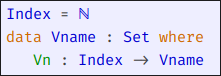
\includegraphics[scale=0.8]{images/IMP/Vname.png}
\end{figure}

\nt{Negli esempi presentati assumeremo X = \texttt{Vn 0}, Y = \texttt{Vn 1} e Z = \texttt{Vn 2}.}

\dfn{Confronto}{
  Per confrontare due variabili definiamo la funzione \texttt{x =Vn y} che compara due nomi e restituisce \texttt{true} se sono gli stessi, \texttt{false} altrimenti. Questa funzione dipende a sua volta da un'altra funzione \texttt{x $=\bbN$ y} per controllare che due $\bbN$ siano uguali.
}

\begin{figure}[h]
  \centering
  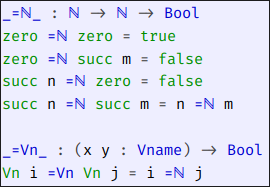
\includegraphics[scale=0.8]{images/IMP/Confronto.png}
\end{figure}


\subsection{Espressioni aritmetiche}

\dfn{Aexp}{
  Si può definire la sintassi delle \evidence{espressioni aritmetiche} (\texttt{Aexp}) con la grammatica:

  \begin{center}
    \texttt{Aexp} $\in$ a, a' ::=  \evidence{N} n | \evidence{V} vn | \evidence{Plus} a a' 
  \end{center}
  Dove n $\in$ \texttt{Nat} e vn $\in$ \texttt{Vname}.
}

\begin{figure}[h]
  \centering
  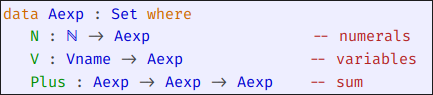
\includegraphics[scale=0.75]{images/IMP/Aexp.png}
\end{figure}

\ex{X + (1 + Y)}{
  aexp0 : \texttt{Aexp}

  aexp0 = Plus (V X) (Plus (N 1) (V Y))
}

\dfn{Stato}{
  Uno \evidence{stato} è una mappatura dai nomi delle variabili ai loro valori:
  \begin{itemize}
    \item [$\Rightarrow$] \texttt{Val} = $\bbN$;
    \item [$\Rightarrow$] \texttt{State} = \texttt{Vname} $\to$ \texttt{Val}. 
  \end{itemize}

  Il significato di stato è un'astrazione della memoria finita di un computer.

}

\nt{Usando questa definizione di stato (che è totale) non si avrà a che fare con funzioni parziali o con il costruttore \texttt{Maybe}.}

\dfn{Aggiornamento}{
L'\evidence{aggiornamento dello stato} è un cambiamento del significato delle singole variabili.

Per formalizzare: l'operatore s [ x ::= v] restituisce lo stato che si comporta come s, ma quando è applicato a X lo trasforma in Y.
}

\begin{figure}[h]
  \centering
  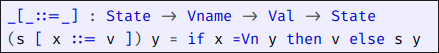
\includegraphics[scale=0.8]{images/IMP/Update.png}
\end{figure}

\ex{Stati}{
\begin{center}
  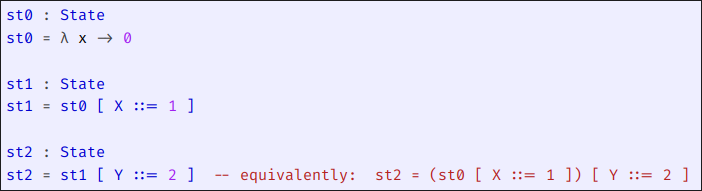
\includegraphics[scale=0.6]{images/IMP/Stati.png}
\end{center}
}

\dfn{Aval}{
  La funzione \texttt{aval} è un'interpretazione di \texttt{Aexpr} utilizzando gli stati.
}

\begin{figure}[h]
  \centering
  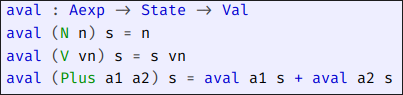
\includegraphics[scale=0.6]{images/IMP/Aval.png}
\end{figure}

\begin{itemize}
  \item Il caso \fancyglitter{N} n non dipende dallo stato, ma restituisce solo n;
  \item Il caso \fancyglitter{V} vn restituisce il valore dello stato s quando applicato a vn\footnote{Ovvero il suo valore salvato in memoria, come nei registri in Assembly.};
  \item Il caso \fancyglitter{Plus} a1 a2 restituisce la somma aritmetica della valutazione ricorsiva su a1 e a2. 
\end{itemize}

\subsection{Sostituzione}

\dfn{Sostituzione}{
  La \evidence{sostituzione} consiste nel rimpiazzare ogni occorrenza di una varibile x in un'espressione a con un espressione a'.
}

\begin{figure}[h]
  \centering
  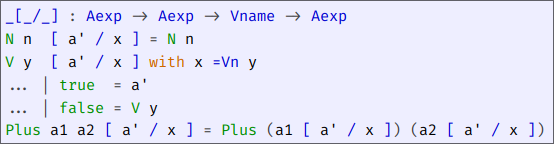
\includegraphics[scale=0.7]{images/IMP/Sostituzione.png}
\end{figure}

\ex{(X + (1 + Y)) [ (Z + 3) / X ]}{
  aexp1 : \texttt{Aexp}

  aexp1 = aexp0 [ Plus (V Z) (N 3) / X ]
}

\mlenma{Sostituzione}{
  Sostituendo x con a' in a e valutando il risultato si ottiene lo stesso stato s che si otterrebbe valutando x nello stato s [ x ::= (aval a' s) ], ossia lo stato in cui il valore di x è stato aggiornato con il valore di a'.
}

\begin{figure}[h]
  \centering
  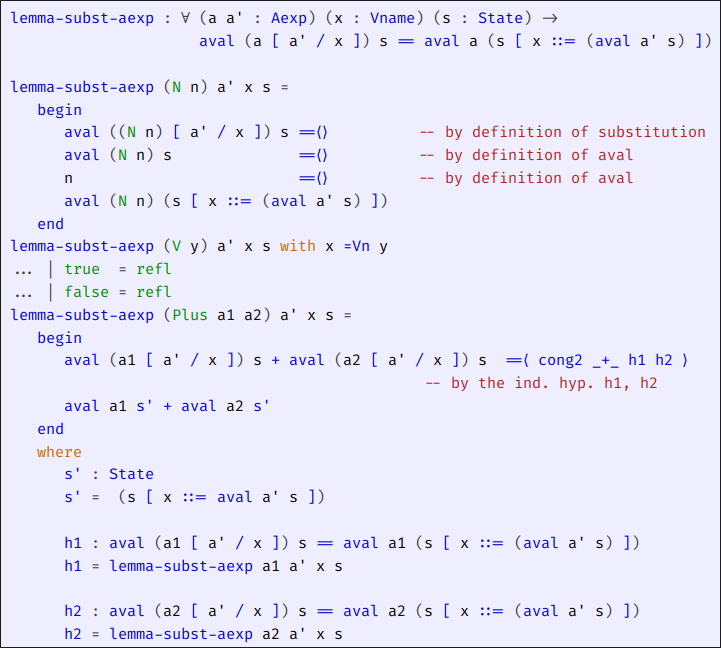
\includegraphics[scale=0.5]{images/IMP/Lsub.png}
\end{figure}

\paragraph{Step della prova:}

\begin{enumerate}
  \item Per prima cosa si fa induzione su a;
  \item Il caso a = \fancyglitter{N} n: banale, perchè non può comparire la x essendo n un numerale;
  \item Il caso a = \fancyglitter{V} y: viene risolto mediante l'utilizzo del costrutto \texttt{with};
  \item Il caso a = \fancyglitter{Plus} a1 a2: si utilizzano le ipotesi induttive perchè ne è la diretta conseguenza.
\end{enumerate}

\subsection{Espressioni booleane}
\dfn{Bexp}{
  Si può definire la sintassi delle \evidence{espressioni aritmetiche} (\texttt{Aexp}) con la grammatica:
  
  \begin{center}
  \texttt{Bexp} $\in$ b, b' ::= B bc | \evidence{Less} a a' | \evidence{Not} b | \evidence{And} b b'
  \end{center}
  Dove bc $\in$ \texttt{Bool} e a, a' $\in$ \texttt{Aexp}.
}

\begin{figure}[h]
  \centering
  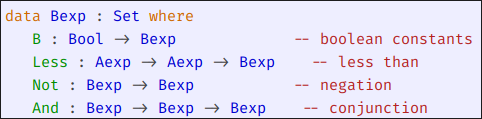
\includegraphics[scale=0.75]{images/IMP/Bexp.png}
\end{figure}

\ex{Alcuni esempi}{
  bexp1 : \texttt{Bexp}

bexp1 = Not (Less (V X) (N 1))      

\subsubsection{}

bexp2 : \texttt{Bexp}

bexp2 = And bexp1 (Less (N 0) (V Y)) 
}

\dfn{Confronto}{
  La valutazione delle espessioni booleane dipende dalla valutazione delle espressioni aritmetiche e quindi, indirettamente, dallo stato.
}


\begin{figure}[h]
  \centering
  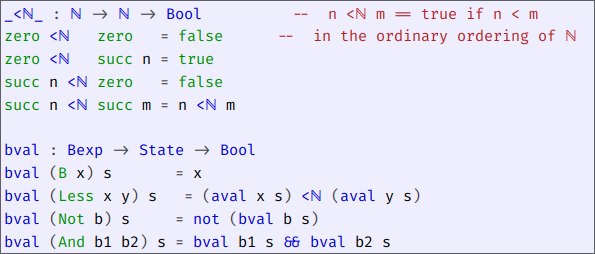
\includegraphics[scale=0.75]{images/IMP/Confronto1.png}
\end{figure}

\pagebreak

\section{Semantica Big-step}

Tra le due possibili semantiche operazionali la Big-step è un approccio astratto basato sulla nozione di \fancyglitter{convergenza}. 

\subsection{Comandi}

\dfn{Comandi}{
  La sintassi dei \evidence{comandi} si basa sulla grammatica:
  \begin{center}
    \texttt{Com} $\in$ c, c' ::= \evidence{SKIP} | x := a | c :: c' | \evidence{IF} b \evidence{THEN} c \evidence{ELSE} c' | \evidence{WHILE} b \evidence{DO} c
  \end{center}

  Dove x $\in$ \texttt{Vname}, a $\in$ \texttt{Aexp} e b $\in$ \texttt{Bexp}.

}

\begin{figure}[h]
  \centering
  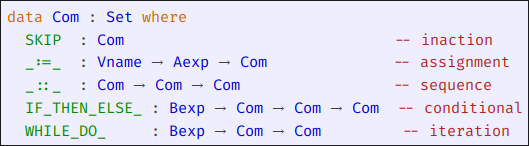
\includegraphics[scale=0.9]{images/IMP/Comandi.png}
\end{figure}

\subsection{Convergenza}

\dfn{Predicato di convergenza}{
  La relazione  $(\!(c , s)\!)  \Rightarrow t$ significa che l'esecuzione di c, quando inizia in s, termina in t. 
}

\nt{
  Questo in generale può richiedere una serie di step che sono racchiusi in un unico Big-step.
}

\cor{Configurazioni}{
  Chiamiamo \evidence{configurazioni} ogni coppia  $(\!(c , s)\!)$ comando-stato. 
}

\begin{figure}[h]
  \centering
  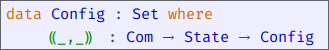
\includegraphics[scale=1]{images/IMP/Configurazioni.png}
\end{figure}

\pagebreak

\dfn{Relazione}{
  Si definisce la relazione $\Rightarrow$ tra \texttt{Config} e \texttt{State} per creare un sistema formale. 
}


\begin{figure}[h]
  \centering
  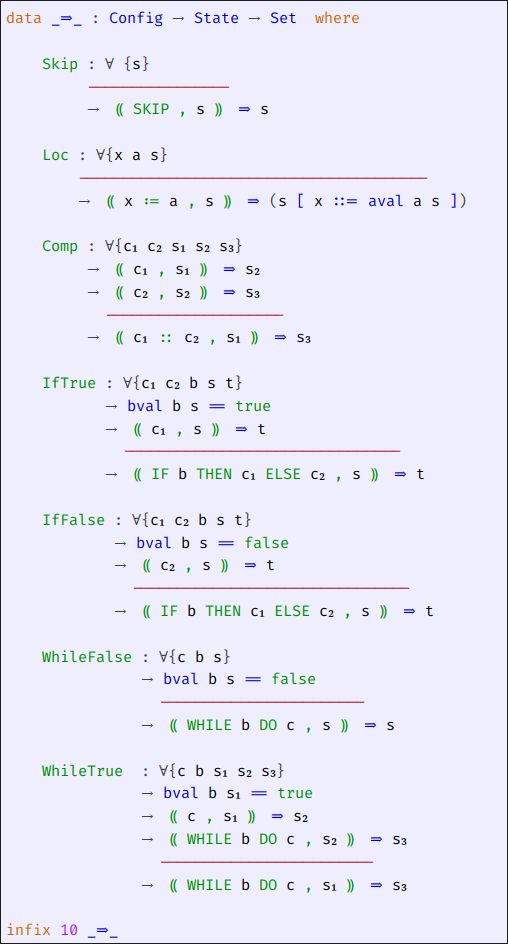
\includegraphics[scale=0.55]{images/IMP/Rel.png}
\end{figure}

\pagebreak

\subsection{Proprietà della convergenza}

\thm{Non trivialità}{
  Esiste almeno un comando che non produce nessuno stato finale come risultato della sua esecuzione.
}

\nt{L'esempio più naturale è \fancyglitter{WHILE} B true \fancyglitter{DO} c.}

\begin{figure}[h]
  \centering
  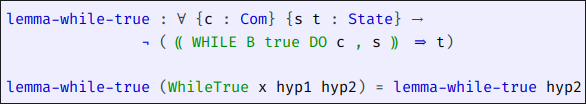
\includegraphics[scale=0.55]{images/IMP/Wtrue.png}
\end{figure}

\begin{itemize}
  \item La prova di questo lemma è per contraddizione;
  \item hyp1 = $(\!(c , s)\!) \Rightarrow s_2$;
  \item hyp2 = $(\!(\text{WHILE B true DO c}, s_2)\!) \Rightarrow t$.
\end{itemize}

\nt{Non è una Reductio Ad Absurdum, ma una semplice prova per contraddizione.}

\thm{Determinismo}{
  Ogni volta che  $(\!(c , s)\!)  \Rightarrow t$ è derivabile per qualche  $(\!(c , s)\!)  \in \text{\texttt{Config}}$ e $t \in$ \texttt{State}, lo stato $t$ è unico.
}

\nt{Per provare questo teorema abbiamo bisogno di due lemmi.}

\mlenma{Una cosa o è vera o è falsa}{

  \begin{center}
    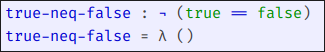
\includegraphics[scale=0.75]{images/IMP/VF.png}
  \end{center}
}

\mlenma{Il vero è diverso dal falso}{

  \begin{center}
    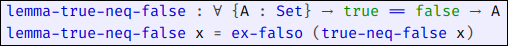
\includegraphics[scale=0.75]{images/IMP/LVF.png}
  \end{center}
}

\pagebreak

  \begin{center}
    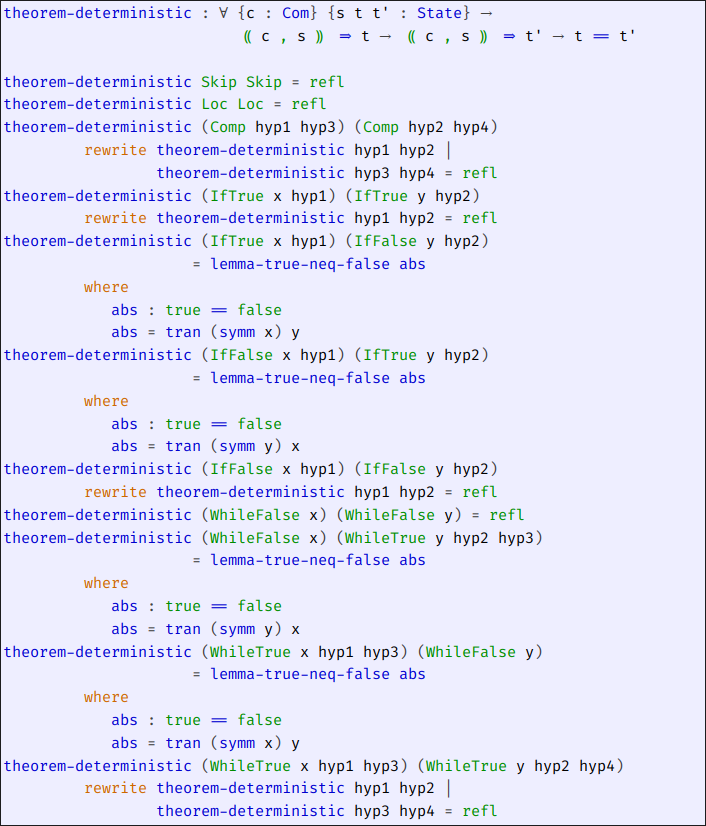
\includegraphics[scale=0.65]{images/IMP/Det.png}
  \end{center}

  \nt{La prova consiste semplicemente in due induzioni simultanee sulle ipotesi $(\!(c , s)\!)  \Rightarrow t$ e $(\!(c , s)\!)  \Rightarrow t'$, usando la tattica \evidence{rewrite}. I due lemmi dimostrati in precedenza sono utili per gestire i casi impossibili riducendoli all'assurdo (ex-falso).}

\subsection{Equivalenza}

\dfn{Equivalenza}{
  Due comandi c, c' $\in$ \texttt{Com} sono equivalenti per ogni s $\in$ \texttt{State} delle computazioni $(\!(c , s)\!)$ e  $(\!(c , s)\!)$ non convergono o $(\!(c , s)\!)  \Rightarrow t$ e  $(\!(c' , s)\!)  \Rightarrow t$  per ogni t $\in$ \texttt{State}. 
}


\begin{center}
 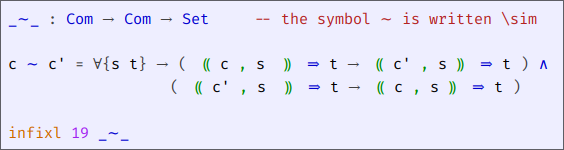
\includegraphics[scale=0.65]{images/IMP/Equivalenza.png}
\end{center}

\nt{L'equivalenza tra i comandi è utilizzata per ottimizzazioni.}

\ex{IF}{

In questo esempio l'IF può essere rimosso perchè sia che la condizione sia vera sia che sia falsa eseguirà sempre lo stesso comando.

  \begin{center}
    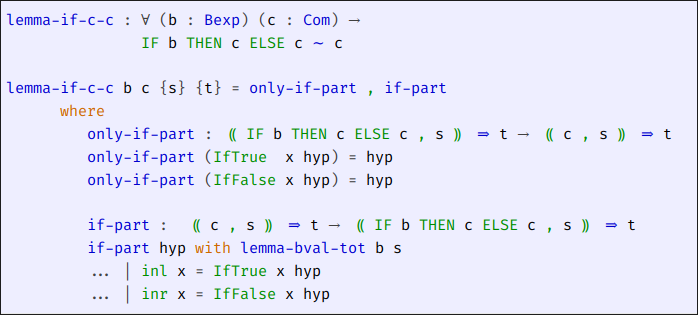
\includegraphics[scale=0.65]{images/IMP/If.png}
  \end{center}

  lemma-bval-tot è un lemma per cui la valutazione di un espressione booleana restituisce o true o false.

}

\pagebreak

\section{Semantica Small-step}

Un approccio alternativo alle semantiche operazionali è quello di descrivere la computazione come l'esecuzione di una serie di step.

\subsection{Riduzione in un passo}

\dfn{Relazione di riduzione in un passo}{
  La relazione $(\!( c , s )\!) \longrightarrow (\!( c' , s' )\!)$ modella l'esecuzione del comando "più a sinistra" in $c$ iniziando da $s$, producendo la nuova configurazione $(\!( c' , s' )\!)$
dove $c'$ (\evidence{continuazione}) è ciò che resta da eseguire di $c$ e $s'$ è il nuovo stato 
prodotto. La relazione $\longrightarrow$ è chiamata \evidence{riduzione in un passo}.

}

\begin{center}
  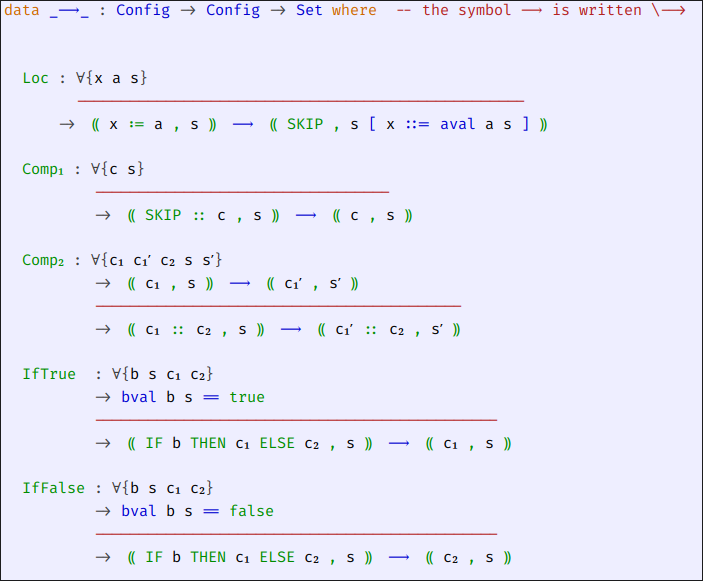
\includegraphics[scale = 0.5]{images/IMP/R1.png}
  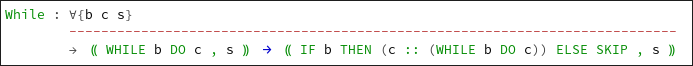
\includegraphics[scale = 0.51]{images/IMP/R2.png}
\end{center}

\begin{itemize}
  \item \fancyglitter{SKIP} è il comando terminale, quindi non riduce a niente e tutti i comandi che lo raggiungono sono terminati;
  \item \fancyglitter{Comp$_1$} indica che il primo comando è terminato e quindi l'esecuzione continua con il prossimo;
  \item \fancyglitter{Comp$_2$} indica che il primo comando si può ridurre a un comando diverso da SKIP;
  \item \fancyglitter{IfTrue} e \fancyglitter{IfFalse} sono banali, perché IfTrue esegue il ramo THEN e IfFalse esegue il ramo ELSE;
  \item \fancyglitter{While} si comporta come in un generico linguaggio di programmazione in cui controlla (mediante If) a ogni iterazione. Se è true continua, mentre se è false diventa SKIP (termina).
\end{itemize}

\pagebreak

\subsection{Chiusure}

\dfn{Riduzione in più passi}{
  La \evidence{riduzione in più passi} (o riduzione) è la chiusura transitiva e riflessiva della riduzione in un passo.
}


\begin{center}
  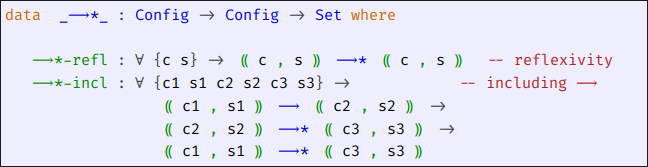
\includegraphics[scale = 0.55]{images/IMP/C1.png}
\end{center}

\begin{itemize}
  \item La regola \fancyglitter{$\longrightarrow$*-refl} postula la riflessività;
  \item La regola \fancyglitter{$\longrightarrow$*-incl} concatena la riduzione in un passo alla riduzione in più passi\footnote{Ricorda il cons nelle liste.}.
\end{itemize}

\nt{Da queste si deriva la regola di transitività.}

\begin{center}
  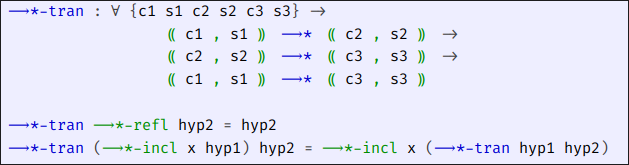
\includegraphics[scale = 0.55]{images/IMP/C2.png}
\end{center}

\paragraph{In AGDA andremo a utilizzare le seguenti macro.}

\begin{center}
  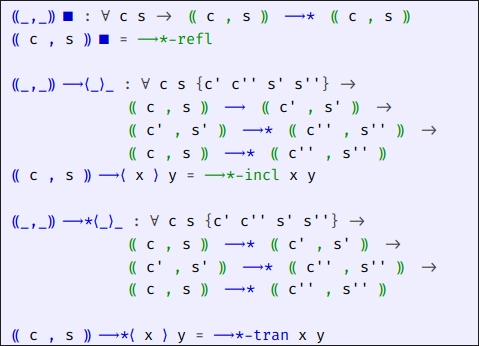
\includegraphics[scale = 0.75]{images/IMP/Macro.png}
\end{center}

\pagebreak

\section{Relazione tra semantica Big-step e semantica Small-step}

\thm{Equivalenza tra Big-step e Small-step}{
  Dati qualsiasi:
  \begin{itemize}
    \item $c \in$ \texttt{Com}.
    \item $s,\;t \in$ \texttt{State}.
  \end{itemize}

  $(\!(c , s)\!)  \Rightarrow t$ se e solo se  $(\!(c , s)\!)  \longrightarrow *(\!(\text{SKIP} , t)\!) $ 

}

\subsection{Da Small-step a Big-step}

\mlenma{Small-Big}{
  Se una configurazione riduce in un passo a un'altra che converge in uno stato allora la configurazione iniziale converge a quello stato.
}

\begin{center}
  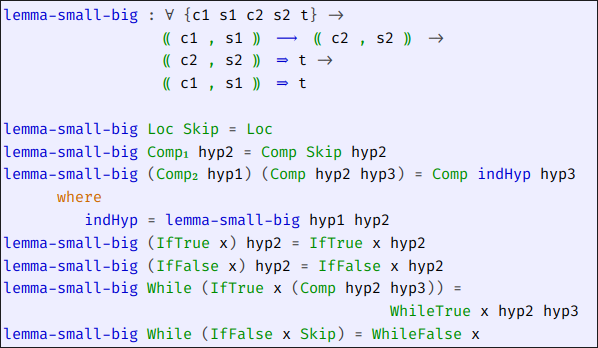
\includegraphics[scale = 0.55]{images/IMP/Small-Big1.png}
  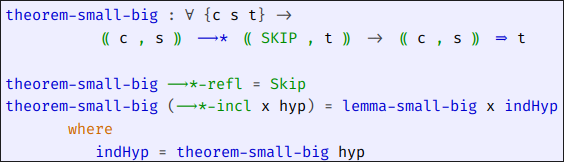
\includegraphics[scale = 0.55]{images/IMP/Small-Big2.png}
\end{center}

\nt{Il teorema Small-Big è una semplice induzione sulla definizione di $\longrightarrow *$.}

\pagebreak

\subsection{Da Big-step a Small-step}

\mlenma{Big-Small}{
  Si estende la regola Comp$_2$ a $\longrightarrow *$ nella definizione di $\longrightarrow$.
}
\begin{center}
  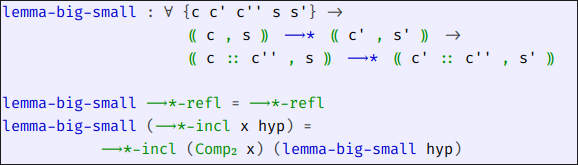
\includegraphics[scale = 0.55]{images/IMP/Big-Small1.png}
\end{center}

\nt{Il teorema Big-Small fa induzione su $(\!(c , s)\!)  \Rightarrow t$ }

\begin{center}
  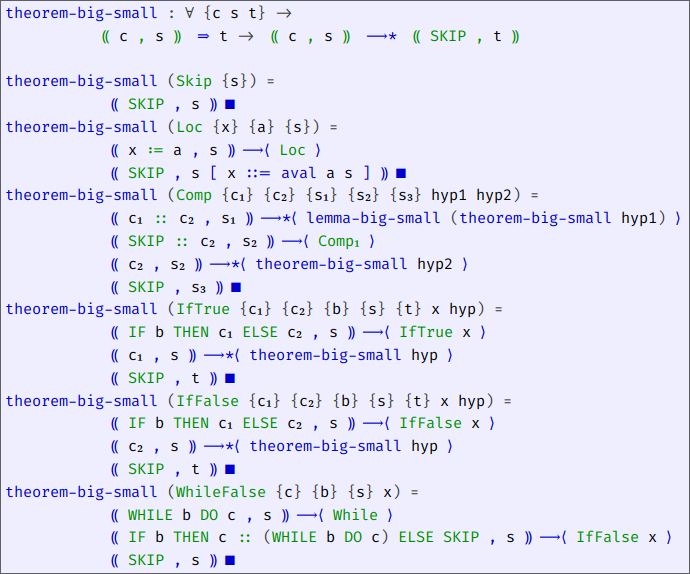
\includegraphics[scale = 0.6]{images/IMP/Big-Small2.png}
  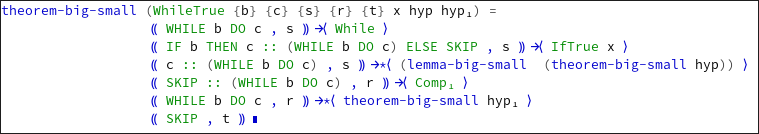
\includegraphics[scale = 0.55]{images/IMP/Big-Small3.png}
\end{center}

\nt{Le due semantiche sono semi-decidibili, ma non decidibili secondo la teoria della computabilità.}


\chapter{Logica di Floyd-Hoare}

\end{document}